
\section{Results and discussion}\label{sec:results}


For each dataset, the combination of the probabilistic degradation model and the SR model (from now on, a pipeline) was trained. 
Each pipeline has 3 main components: 
\begin{itemize}
    \item A generator, used to generate LR images similar to the target domain, from HR images coming from the source domain.
    \item A discriminator, used to distinguish between real and generated LR images.
    \item A SR model, used to super resolve the LR images generated by the generator or the real LR images coming from the target domain.
\end{itemize}

The pipeline trained on $\mathcal{D}_{\text{SF}-\text{SF}}$, using unpaired HR-LR pairs generated by applying the baseline degradation model described in \ref{fig:3-probabilistic-degradation-model} to the synthetic FOREST-2 images, will be referred to as the baseline pipeline.
While the employed degradation model is stochastic, it has known parameters. The objective is to observe how the GAN is able to imitate a known degradation model  in order to produce LR images.

The pipeline trained on $\mathcal{D}_{\text{SF}-\text{RF}}$, using unpaired HR-LR pairs of synthetic and real FOREST-2 images, will be referred to as the adapted pipeline.
In this case, the degradation model is unknown and the objective of the GAN is to to estimate it, generating LR versions of the synthetic FOREST images that come from the same distribution as the real FOREST images.

    \subsection{Source domain}

        This subsection will analyze the results from the experiments performed on the source domain.
        The process consists of degrading the synthetic HR FOREST images using the generator trained using adversarial learning and then super resolving it using the corresponding SR model from the pipeline.
        This is the equivalent of the black arrows flow described in fig. \ref{fig:3-GAN-degradation-model}. 
        As in this case the ground truth is known, the performance of the super resolution can be evaluated using metrics like PSNR and SSIM. 

        Fig. \ref{fig:5-source_domain_sample} shows the results of the baseline and the adapted pipeline, when applied to one sample from the source domain (a synthetic HR FOREST-2 image). 
        For comparison, a pipeline consisting of simple gaussian blurring + downscaling for degradation and bicubic upsampling for SR is also shown. 

        While the baseline kernel is very simple and the noise is more or less uniform across the image, the adapted kernel is more complex and the noise seems to be strongly correlated with the image intensity.
        It is important not to overinterpret this result, as the kernel and noise are estimated using overparametrized models, and multiple combinations of kernel and noise may produce similar results. 
        However, it is interesting to see that the adapted pipeline is able to estimate a more complex degradation model, which is closer to the real degradation model used in the target domain.

        The degraded LR images present considerable differences. While the baseline pipeline produces images very similar to gaussian blurring + downscaling, 
        the adapted pipeline produces much more blurry images with more noise, suggesting that FOREST-2 produces less resolution than what was initially expected. 
        This is also confirmed by calculating the PSNR between the LR image generated by each pipeline with the gaussian blurring + downscaling LR image, which yields worse results for the adapted pipeline.
        
        The super resolved produces by both pipelines yield better performance than bicubic interpolation, and they are very similar between them.
        This suggests that the super resolution model is able to recover the details lost during a more complex degradation processes, but there seems to be a limit to the amount of detail that can be recovered. 
        It is observed that even though the starting point is different ( baseline LR is less blurry than adapted LR), the final result is very similar.

        
        
        
        \begin{figure}[H]
            \centering
            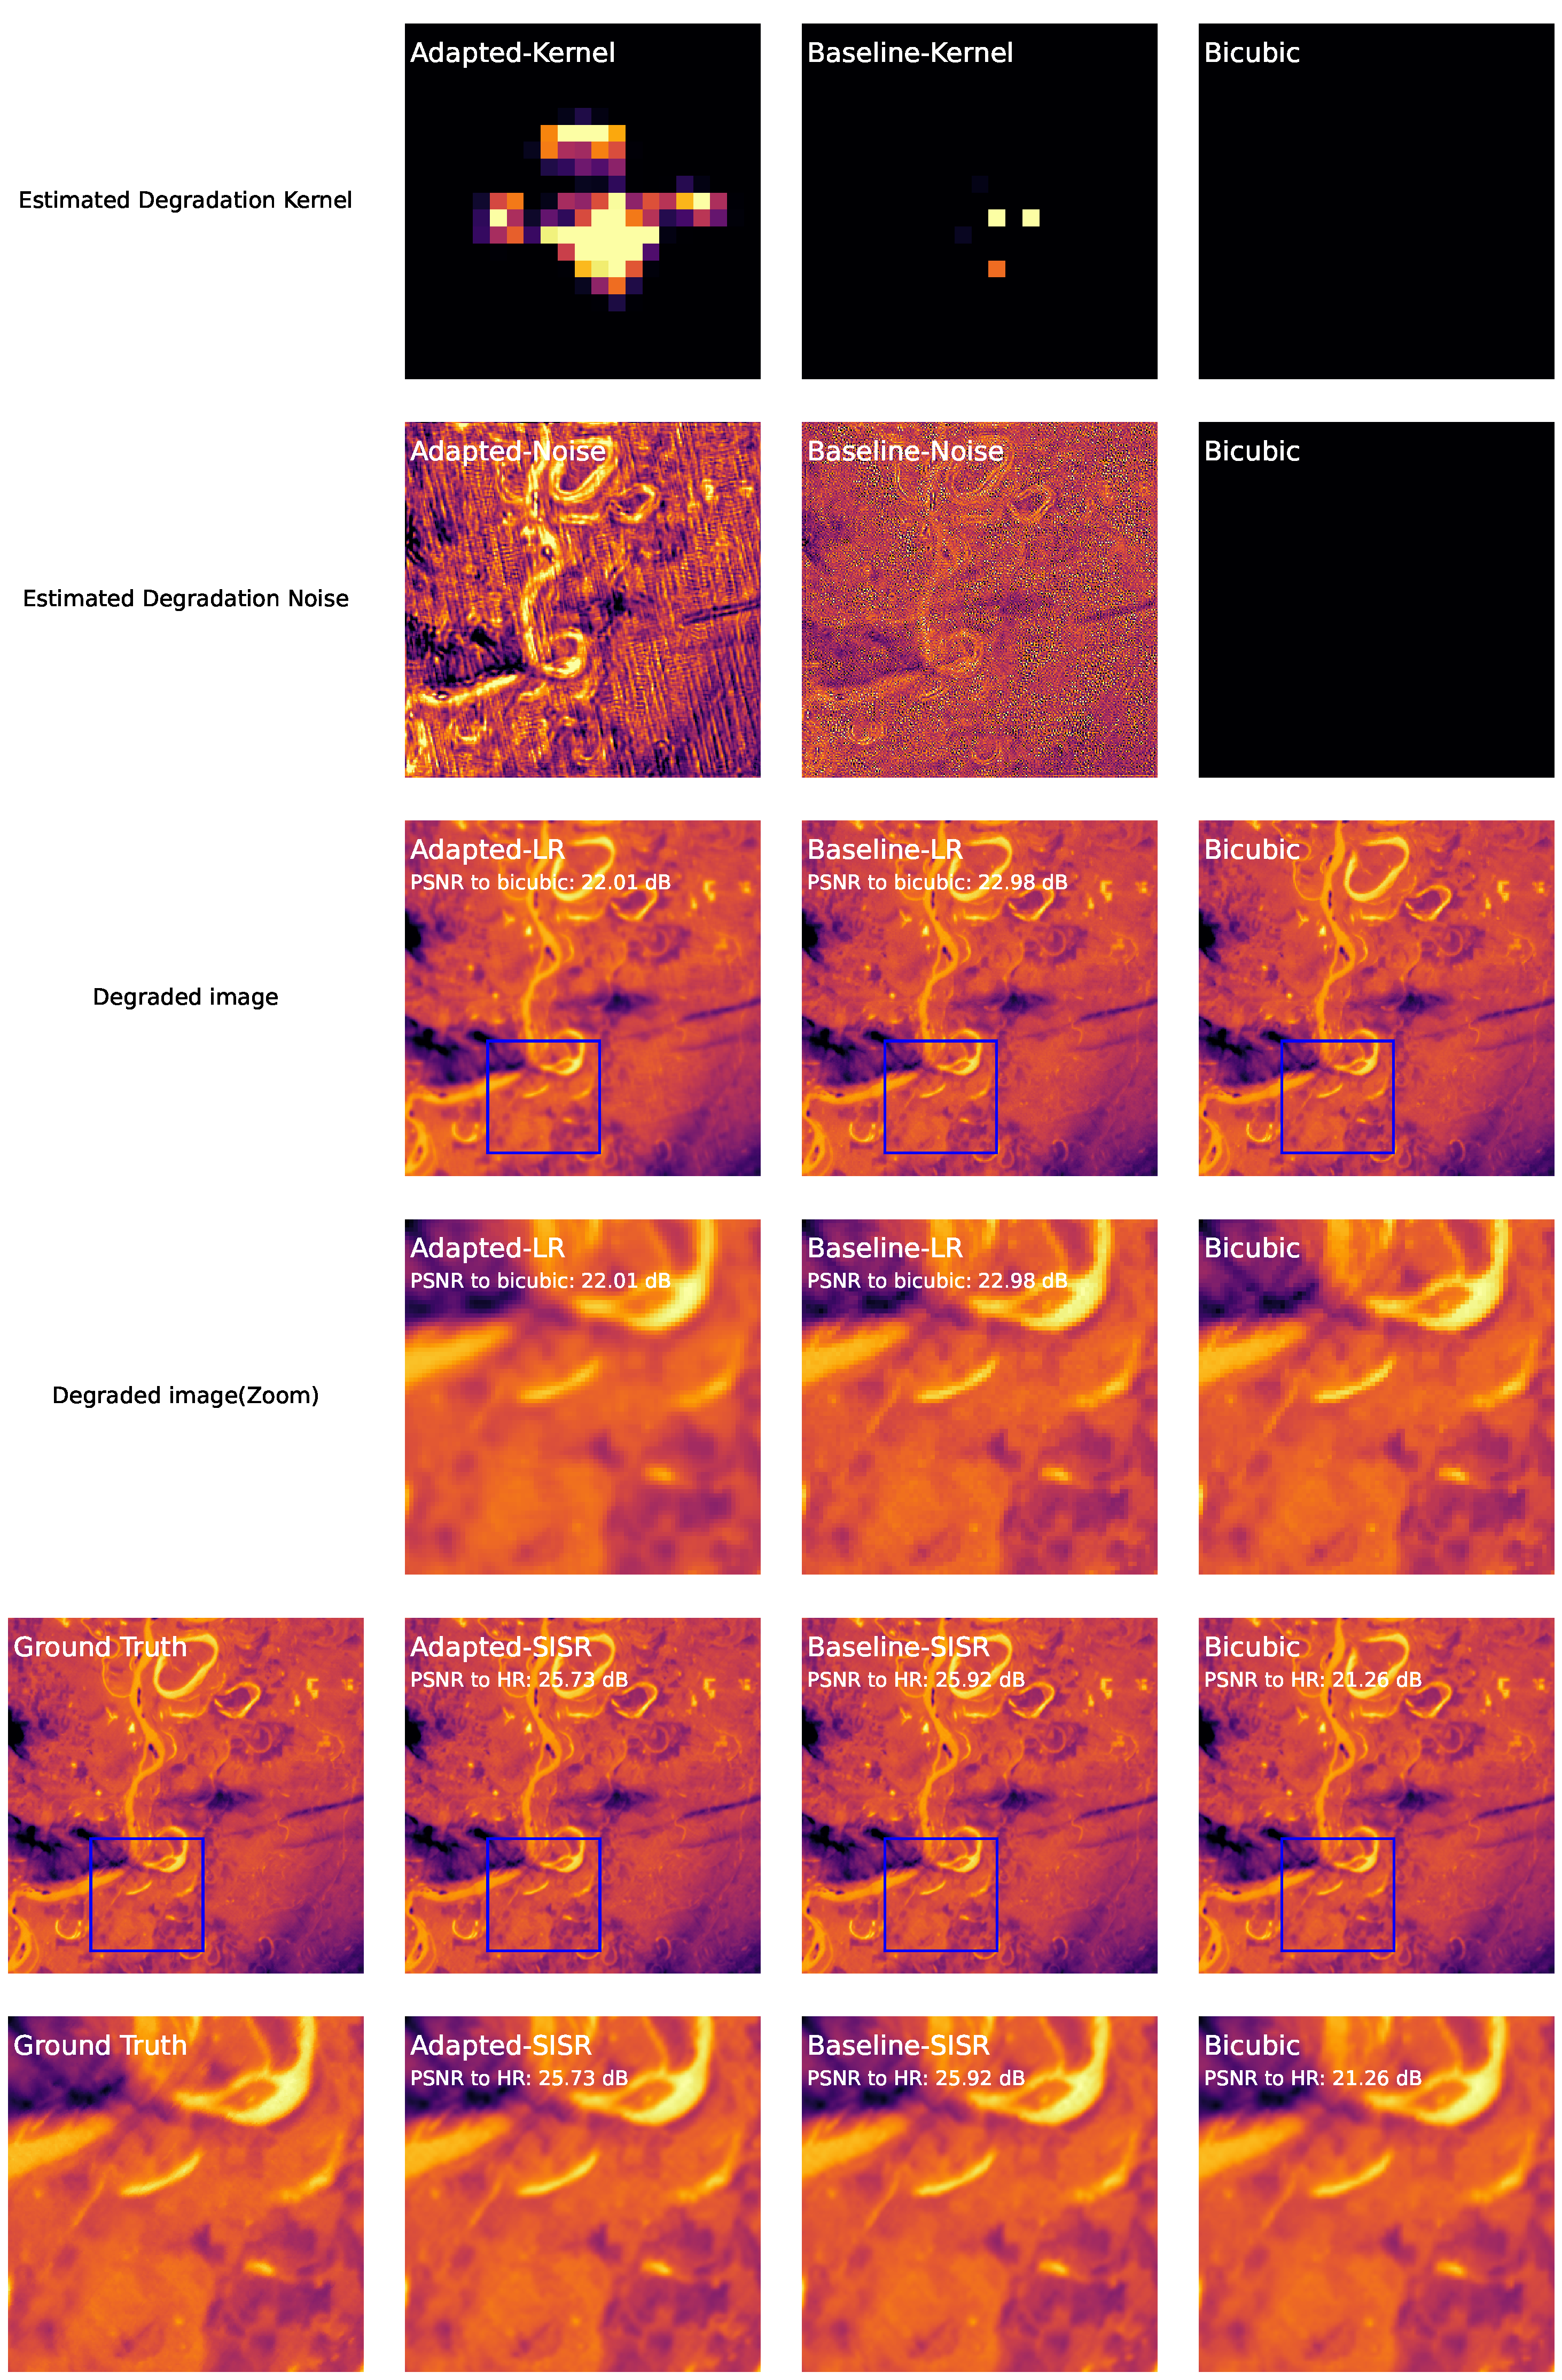
\includegraphics[width=\textwidth]{Includes/5-source-prediction-sample.pdf}
            \caption{Applying different degradation models on an HR sample. 
                     The 2 most upper rows show the estimated degradation kernels and noise of each pipeline, the bicubic downsampling does not estimate a kernel or noise.
                     The degraded LR images from each model and a zoom is displayed on the two subsequent rows. 
                     In this case, the PSNR is calculated against the gaussian blurring + bicubic downsampling LR.
                     The synthetic FOREST-2 (ground truth) and the super resolved images, with a zoom, are displayed in the last 2 rows. 
                     The PSNR for each SR method is calculated against the HR synthetic FOREST-2.
            }
            \label{fig:5-source_domain_sample}
        \end{figure}


        In Figs \ref{fig:5-lr-images-fft.pdf} the frequency domain of the LR images is analyzed.
        By inspection of the FFTs, it is observed that the adapted-LR loses more information than the baseline-LR, as the log magnitude of the FFT get cut more close to the center.
        The baseline-LR FFT is very close to the gaussian blurring + bicubic upsampling FFT, suggesting that the baseline pipeline is able to mimic this known degradation model.

        \begin{figure}[H]
            \centering
            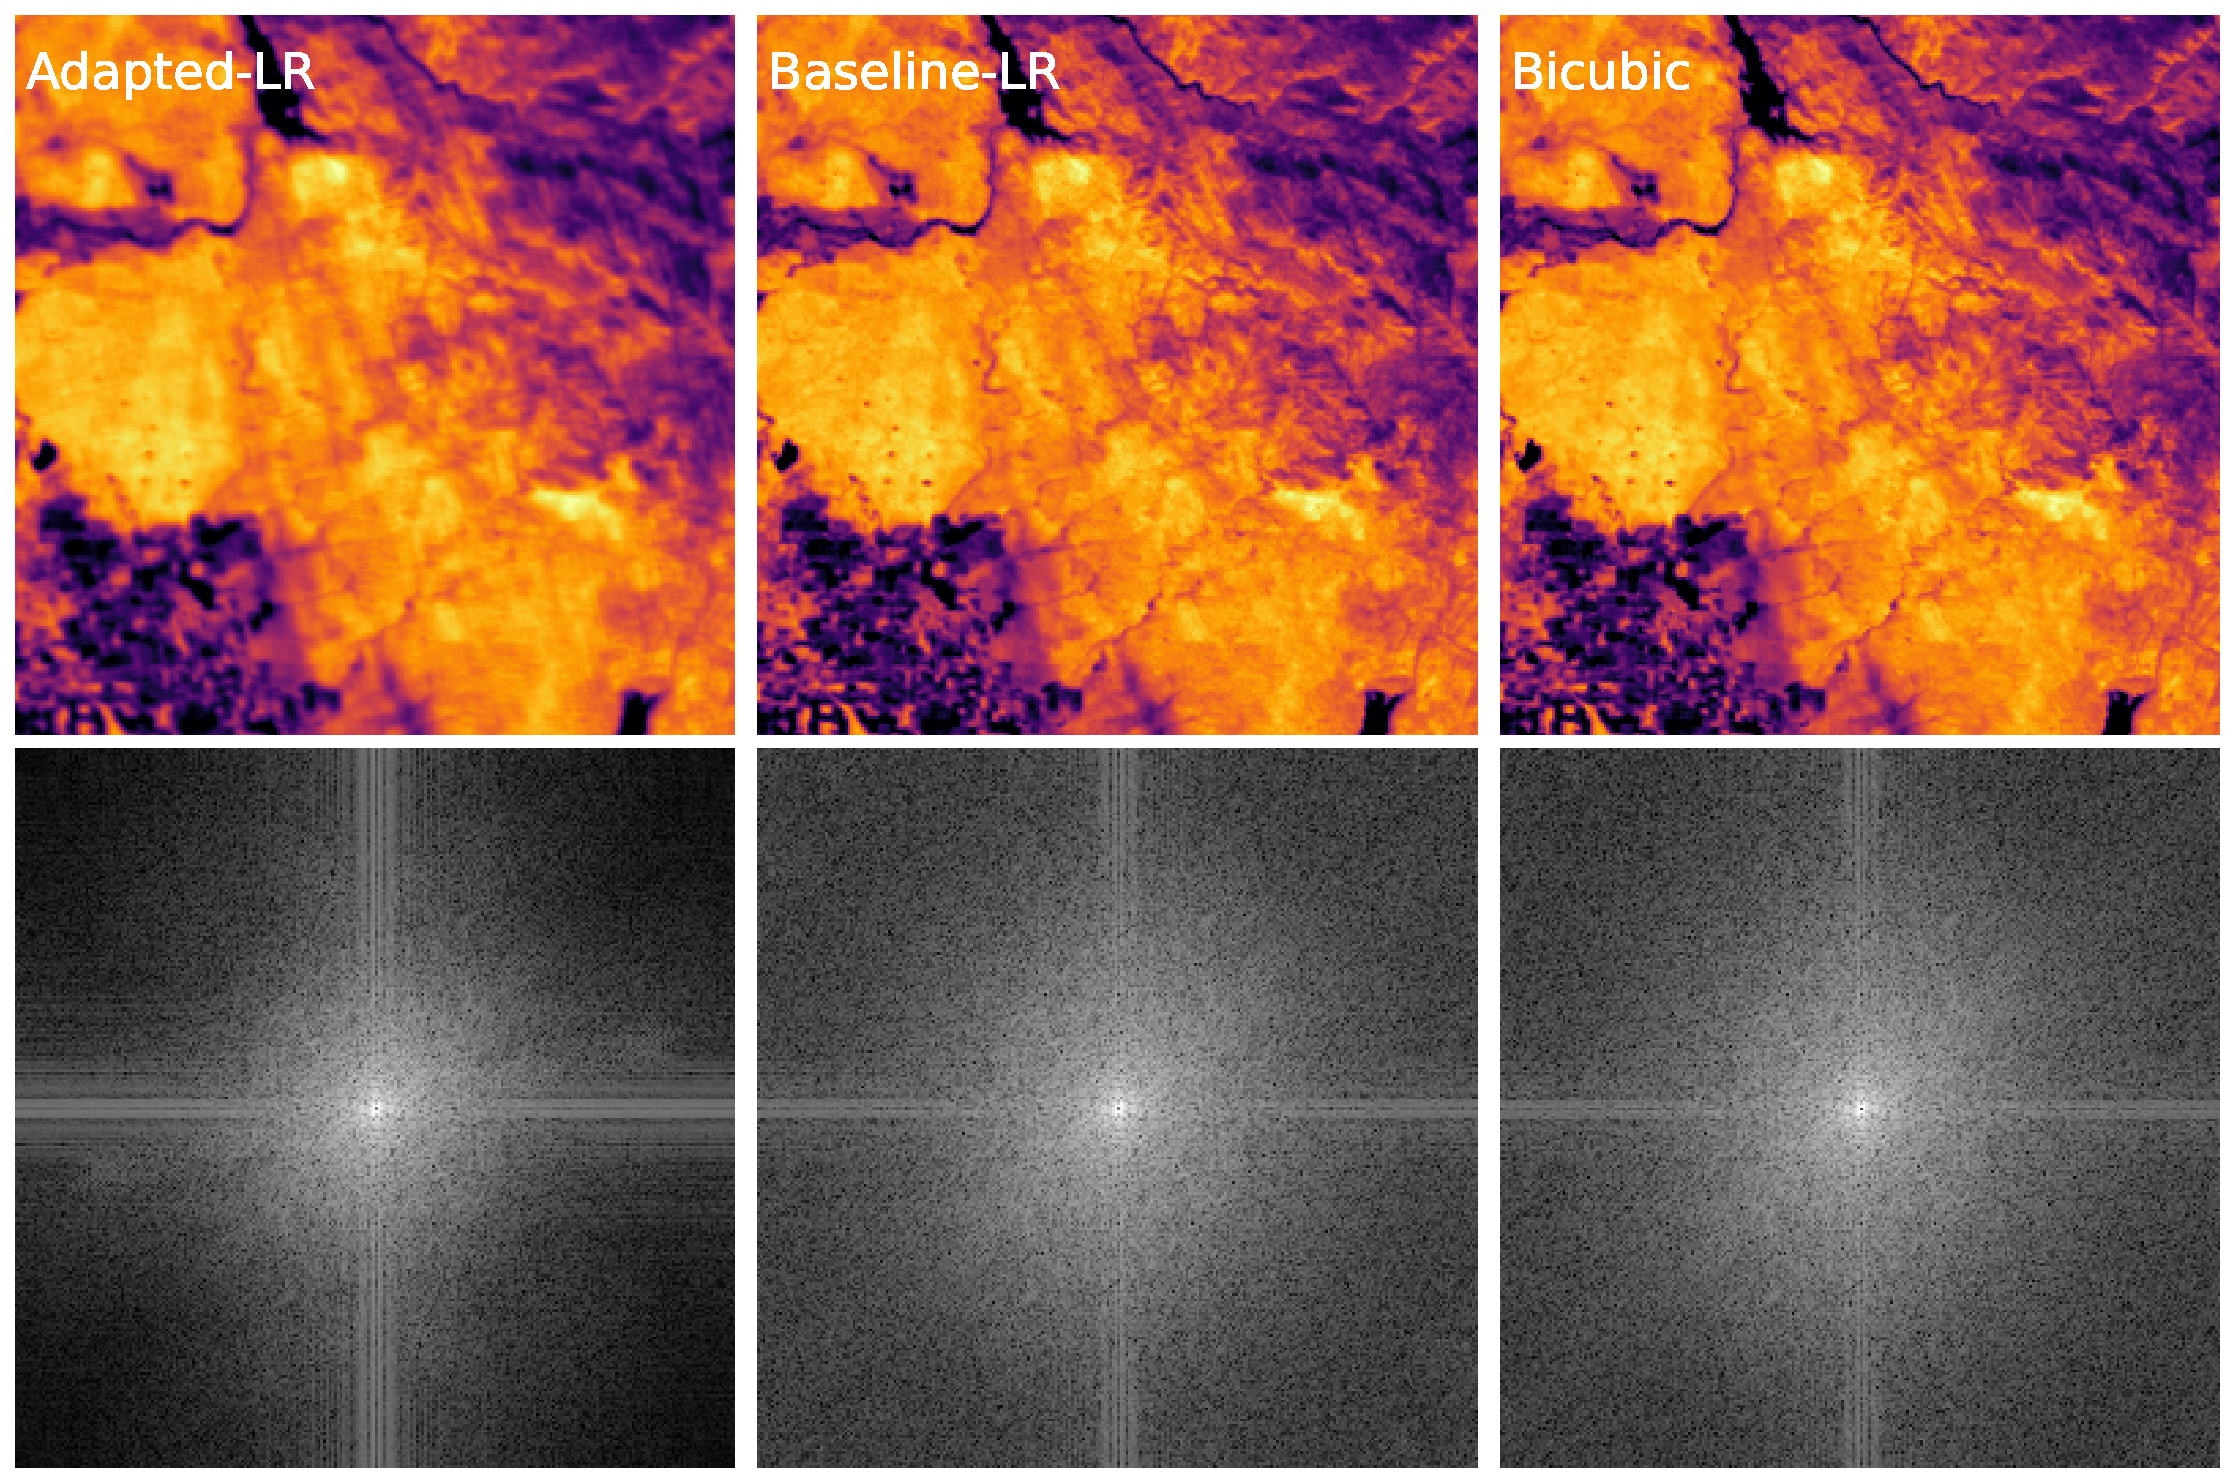
\includegraphics[scale=0.3]{Includes/5-lr-images-fft.pdf}
            \caption{Log mangnitude of the FFT for the LR images obtained by the pipelines and the gaussian blurring + bicubic upsampling.}
            \label{fig:5-lr-images-fft.pdf}
        \end{figure}

        The radial profile of the log magnitude of the FFT for the LR images shown in Fig. \ref{fig:5-lr-images-fft-comparison.pdf} confirmed what was observed previously.
        The adapted-LR image diminishes the high frequency components much more than the baseline-LR image with amplifications of -6dB in frequencies starting at 0.1 cycles per pixel, with a stable effect of -6dB from 0.3 to 0.7 cycles per pixel. 
        It is important to note that 0.1 cycles per pixel at a 210m GSD corresponds to a cycle frequency of 2100m, 0.3 cycles per pixel corresponds to 700m and 0.7 cycles per pixel to 300m.
        This suggests that the degradation model from the real FOREST-2 images is more complex and loses more information than the baseline degradation model.
        An analysis for the whole validation dataset will be further discussed to verify that this behaviour is consistent across different scenes and conditions.


        \begin{figure}[H]
            \centering
            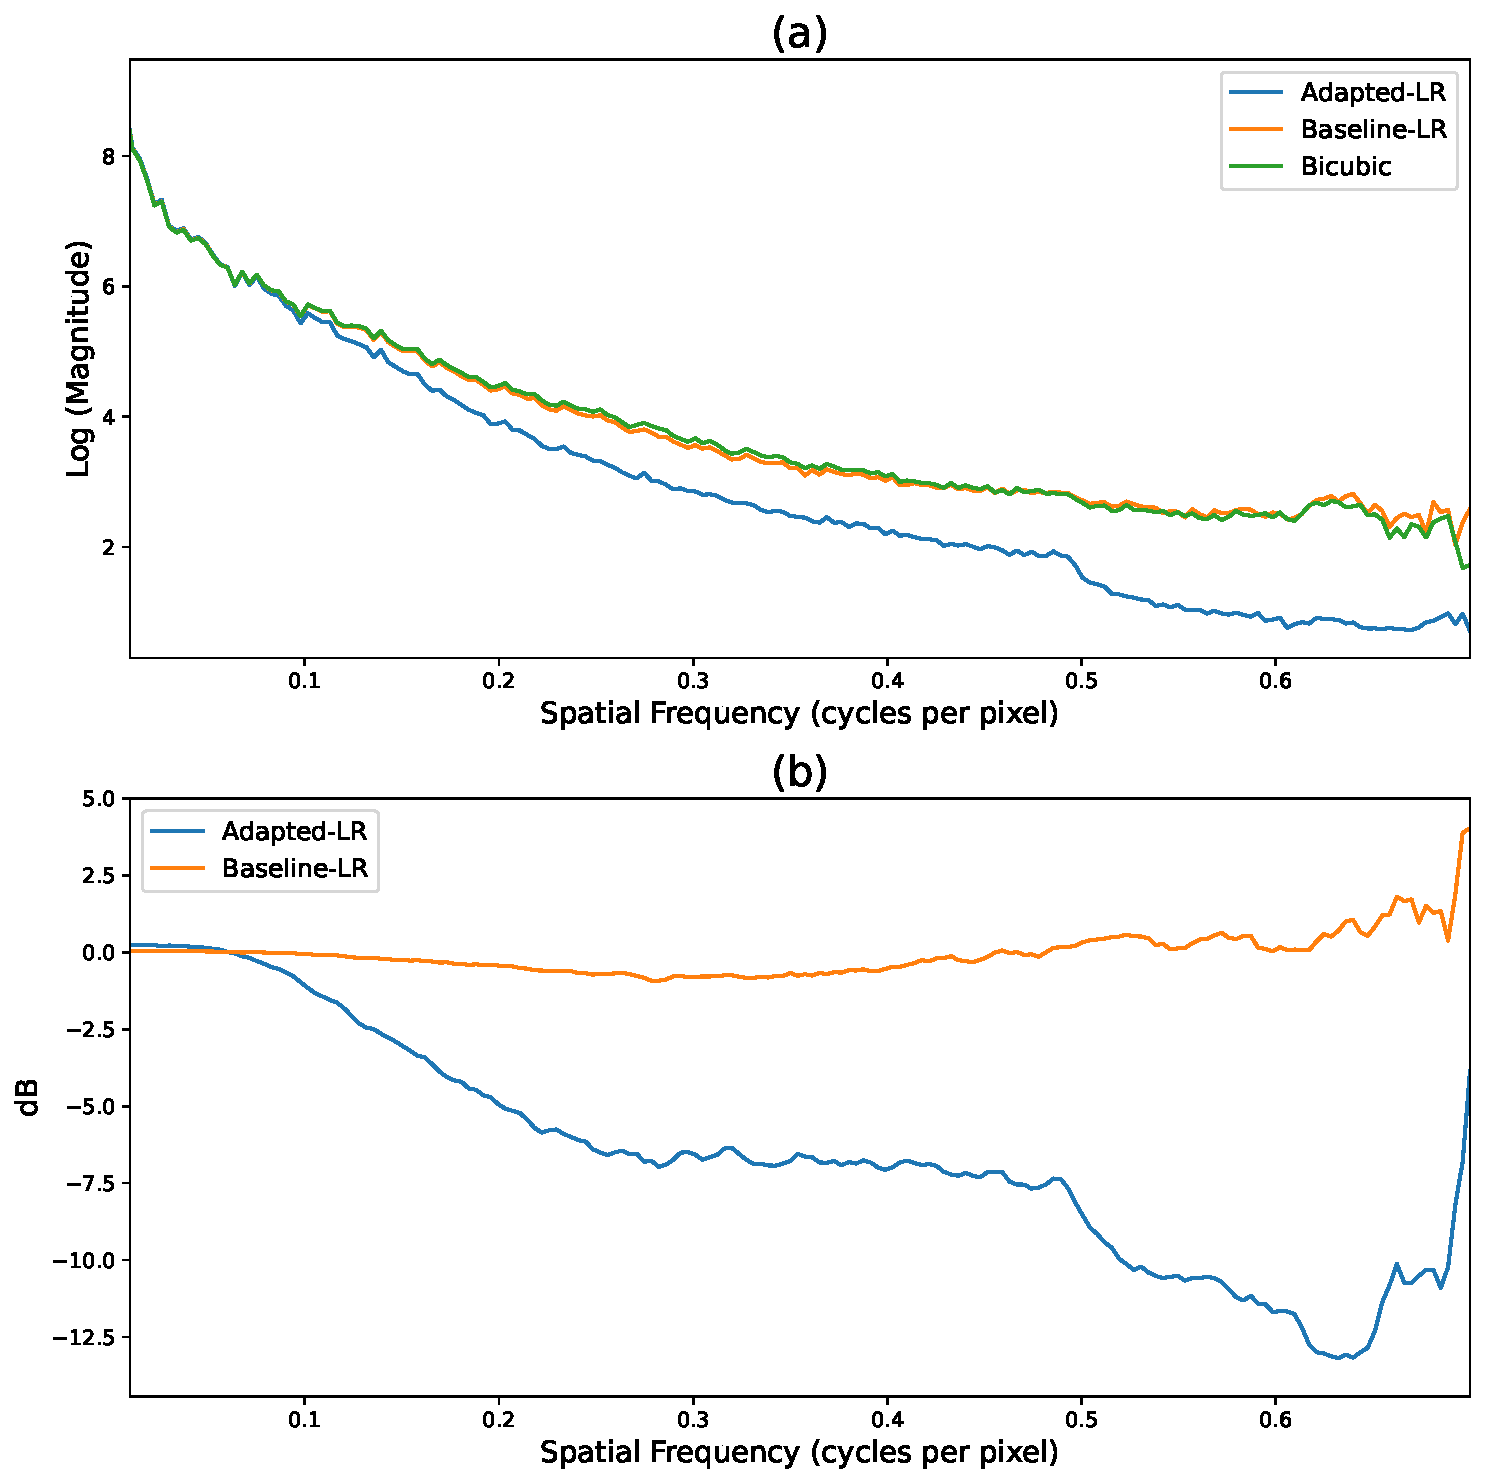
\includegraphics[scale=0.45]{Includes/5-lr-images-fft-comparison.pdf}
            \caption{(a) Radial profile of the log magnitude across spatial frequency of the LR images obtained by the pipelines and the gaussian blurring + bicubic downsampling model.
                     (b) Amplification in dB of each pipeline with respect to the gaussian blurring + bicubic downsampling.}
            \label{fig:5-lr-images-fft-comparison.pdf}
        \end{figure}

        When analyzing the super resolved images versus the ground truth in the frequency domain, a very similar frequency response is observed for the super resolved images of the adapted and the baseline pipelines.
        Moreover, the SR images are able to stay above -3dB, a common threshsold used in the literature, up until 0.3 cycles per pixel, which correspond to 300$\frac{1}{m}$ when each pixel equals 70m.
        This suggests that the SR model in the adapted pipeline is able to recover the lost information at those frequencies due its more complex degradation model.
        Starting at 0.3 cycles per pixel, a decrease in amplification is observed for both pipelines, but more steeply for the adapted pipeline.
        This may be related to the fact that the adapted degradation model diminishes cycles at higher frequencies even more than the baseline degradation model. 
        A limit for the SR algorithm is also noted, even using an optimistic degradation model such as the baseline, the SR model is not able to recover higher frequencies with respect to the original, HR image.
        Even if it is slightly better than bicubic upsampling, the diminishing of the higher frequency components is dramatic.

        \begin{figure}[H]
            \centering
            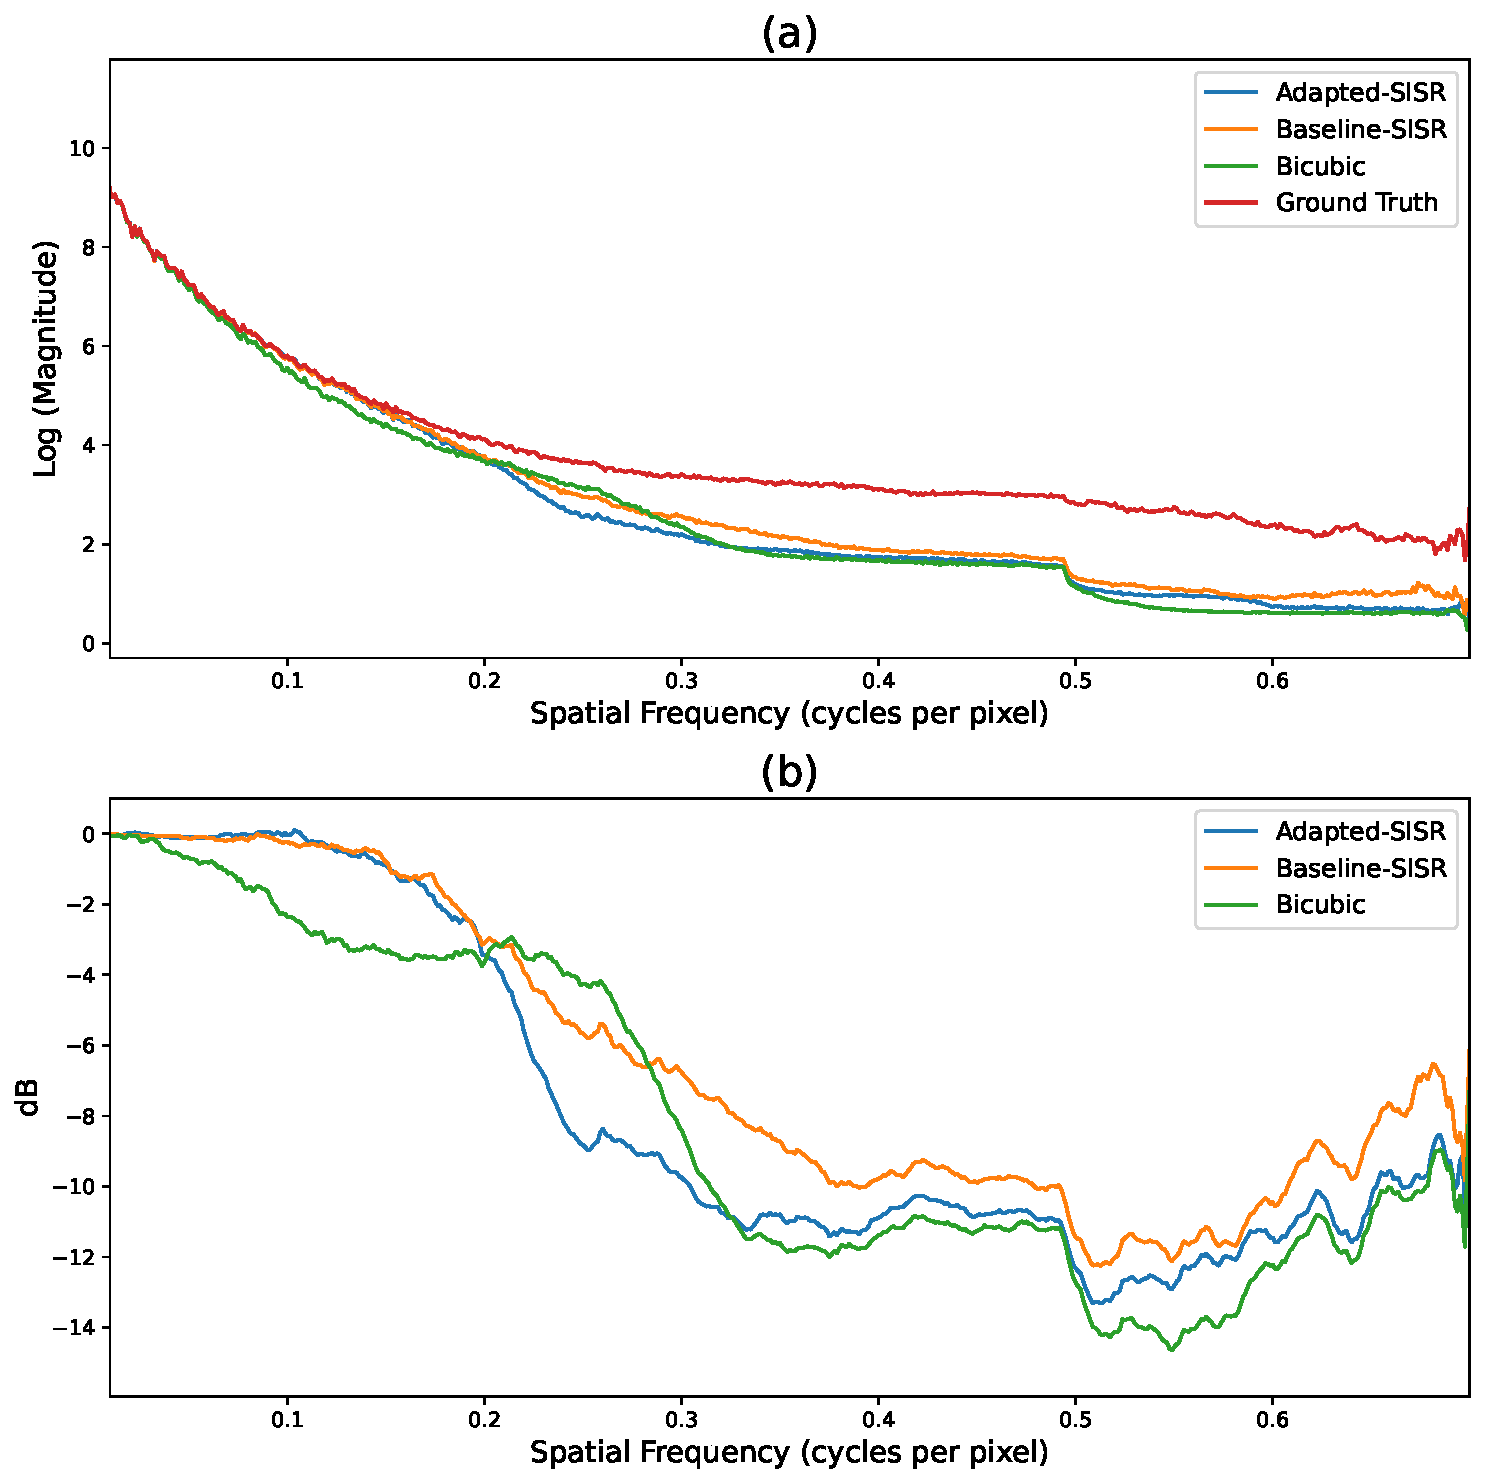
\includegraphics[scale=0.5]{Includes/5-source-sr-fft-comparison.pdf}
            \caption{Frequency domain analysis of the SR images and the ground truth displayed in \ref{fig:5-source_domain_sample}.
                     In (a), the log of the magnitude of the FFT for the SR images and the ground truth is shown,
                     while in (b), the amplification of each SR image with respect to the ground truth is shown.}
            \label{fig:5-source-sr-fft-comparison}
        \end{figure}


        \subsubsection{LR comparison}

        A quantitative analysis of the LR images obtained by the generator of each pipeline is performed. 
        Fig. \ref{fig:5-source-domain-lr-performance-scatterplot} shows 3 supervised performance metrics obtained by comparing the LR images obtained by the pipelines with the gaussian blurring + bicubic downsampling degradation.
        In this case, a consistent higher PSNR and SSIM means that the baseline-LR image is closer to the gaussian blurring + bicubic downsampling LR image than the one generated by the adapted pipeline. 
        A lower LPIPS means that even using perceptual metrics, the baseline-LR image is also closer.
        This is consistent with the results shown in Fig. \ref{fig:5-source_domain_sample}, where the adapted LR image is more blurry and noisy, suggesting that the unknown degradation is worse than the baseline degradation model.
        
        \begin{figure}[H]
            \centering
            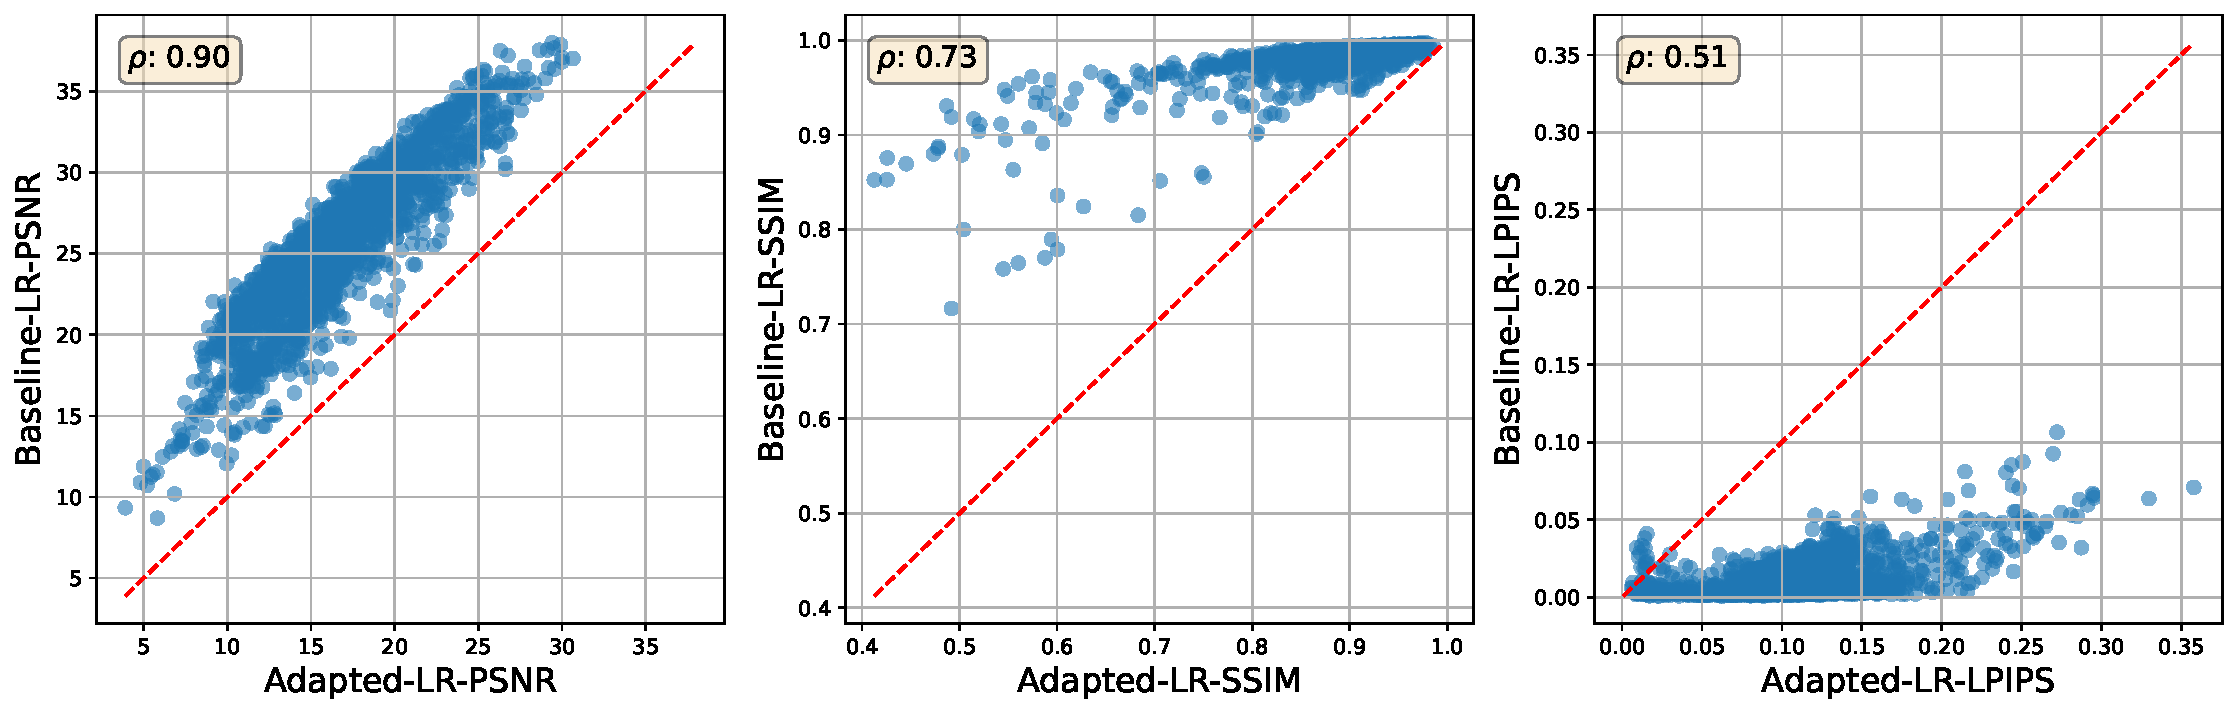
\includegraphics[width=\textwidth]{Includes/5-source-domain-lr-performance-scatterplot.pdf}
            \caption{Performance metrics between the LR images obtained by the pipelines vs the gaussian blurring + bicubic downsampling degradation.}
            \label{fig:5-source-domain-lr-performance-scatterplot}
        \end{figure}




        An alternative way to evaluate the differences in the degradations is by analyzing the frequency domain of the LR images.
        An analysis of the whole validation dataset is performed by calculating the FFT of each LR image and comparing them with the gaussian blurring + bicubic downsmapling degradation model.
        The results are displayed shown in Fig. \ref{fig:5-lr-images-fft-comparison}. 
        In (a) the log magnitude of the FFT across different spatial frequency values for the degraded images is shown. 
        The spatial frequency is obtained from the radial distance to the center of the FFT, as shown in \ref{subsubsec:frequency_domain_analysis}.
        In (b), the amplification of each generated LR image with respect to a simple gaussian blurring + downscaling is shown. 
        The results for the whole dataset show that the LR images generated by the adapted pipeline yield a reduction in the higher frequency components consistently across all samples, with a ± 1 standard deviation interval between -4 and -6 dB from between 0.3 and 0.7 cycles per 210m pixel.
        This translates in blurrier images, and a more difficult starting point for a SR model to work with.

        \begin{figure}[H]
            \centering
            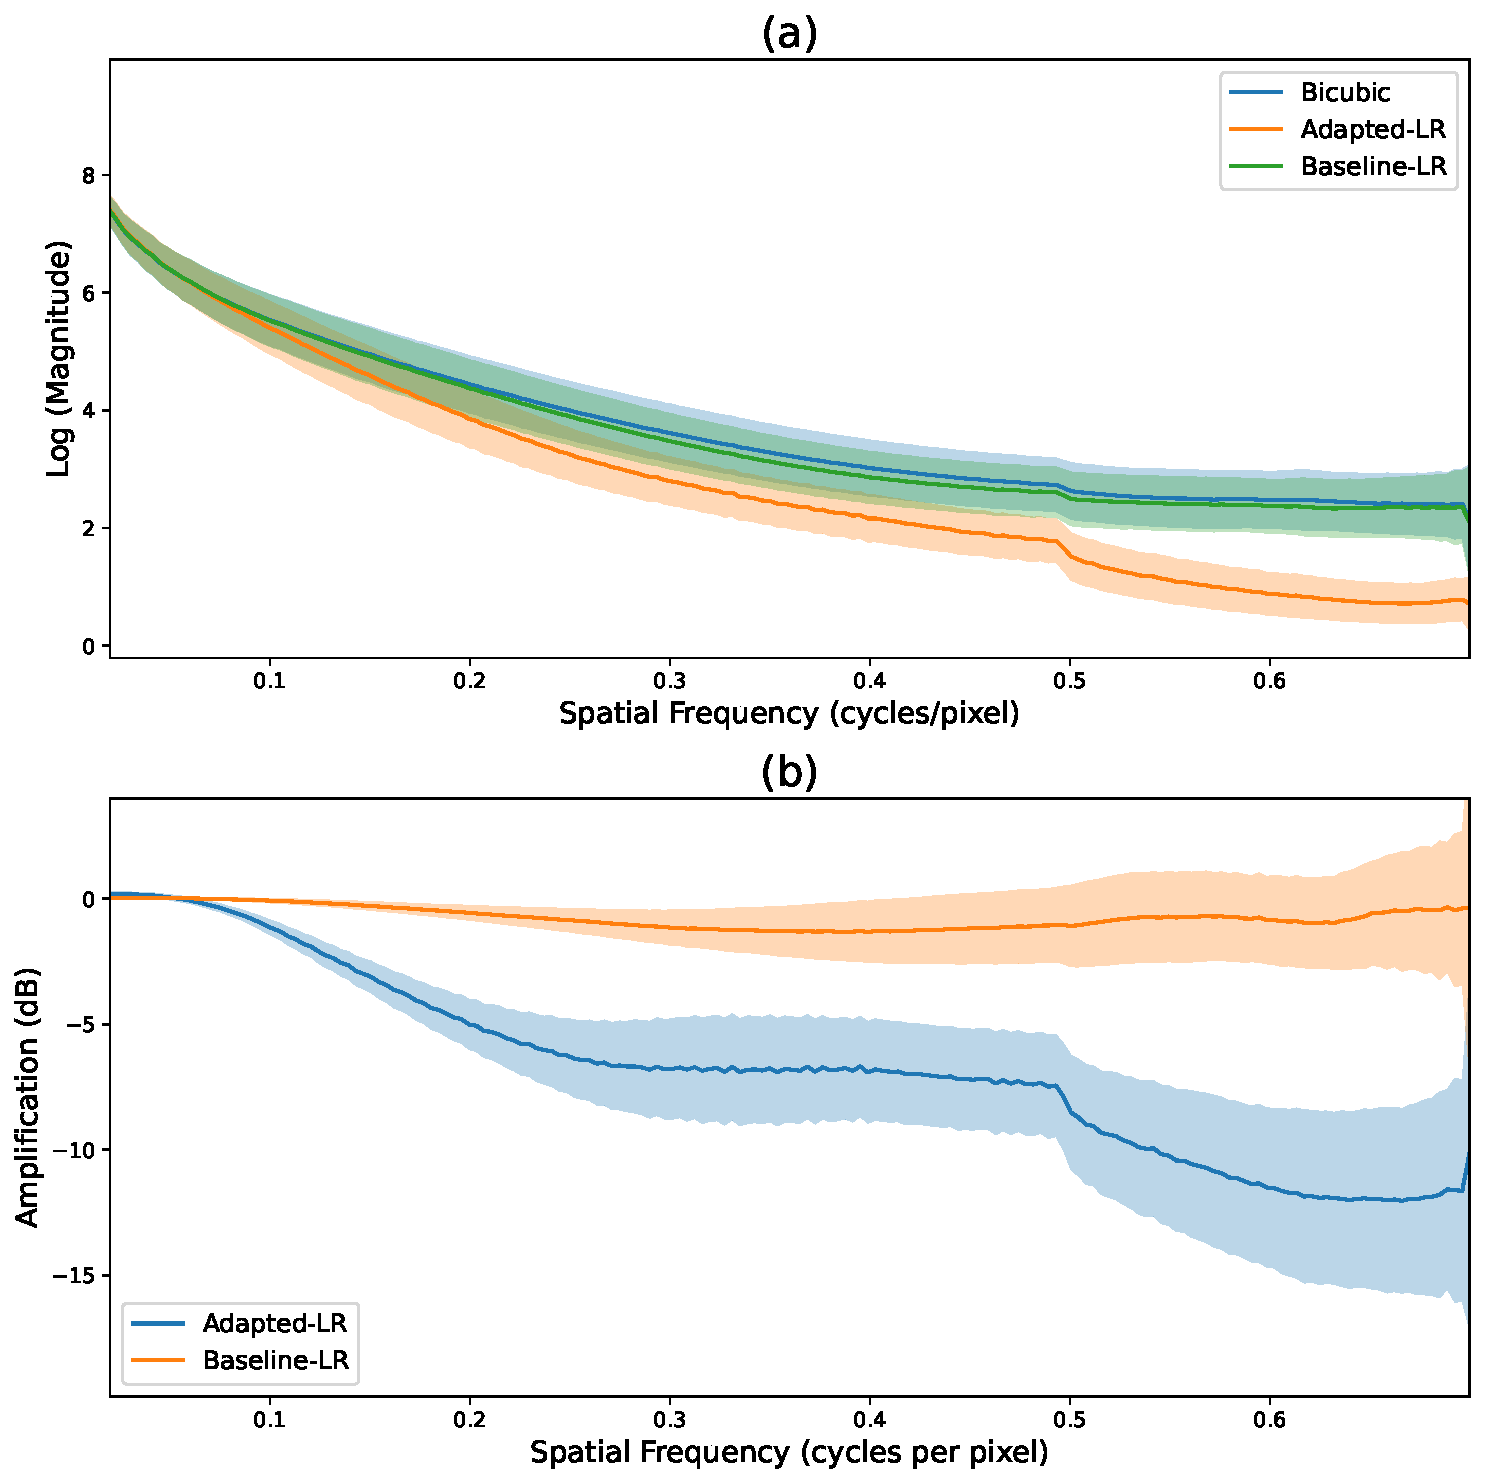
\includegraphics[scale=0.5]{Includes/5-source-lr-amplification-statistics.pdf}
            \caption{Frequency domain analysis of the LR images obtained by applying different degradation models on the HR sample displayed in Fig. \ref{fig:5-source_domain_sample}.
                     In (a), the log of the magnitude of the FFT for the LR images is shown,
                     while in (b), the amplification with respect to a  simple gaussian blurring + downscaling is shown.
                     The painted area represents the ±1 standard deviation of the radial profiles and the amplification. }
            \label{fig:5-lr-images-fft-comparison}
        \end{figure}




        \subsubsection{Effects of the degradation model in SR}

        Another subject of interest is how the degradation model affects the performance of the super resolution process.
        Fig. \ref{fig:5-source-domain-comparison} shows the performance obtained by super resolving the output of each pipeline generator for the whole validation dataset.
        In the upper row (a), the corresponding SR model of each pipeline is used to obtain the super resolved images. 
        The performance, both in PSNR and SSIM, are very similar for both pipelines. The LPIPS shows a consistent behavior too.
        In the lower row (b), the SR model is discarded and a simple bicubic upsampling is used to super resolve the degraded images of each pipeline. 
        In this case, using the baseline LR version as input consistently yields better results than the adapted LR version, in all metrics.
        This suggests that the learned degradation model from FOREST-2 images loses more information than the baseline, resulting in a lower effective ground sampling distance than what was is specified in FOREST-2 fact sheet.
        Consistent with what was found in the frequency domain analysis observed in Fig. \ref{fig:5-source-sr-fft-comparison}, the SR model is able to recover most of the information, as the performance after using the SR models is very similar. 
        
        \begin{figure}[H]
            \centering
            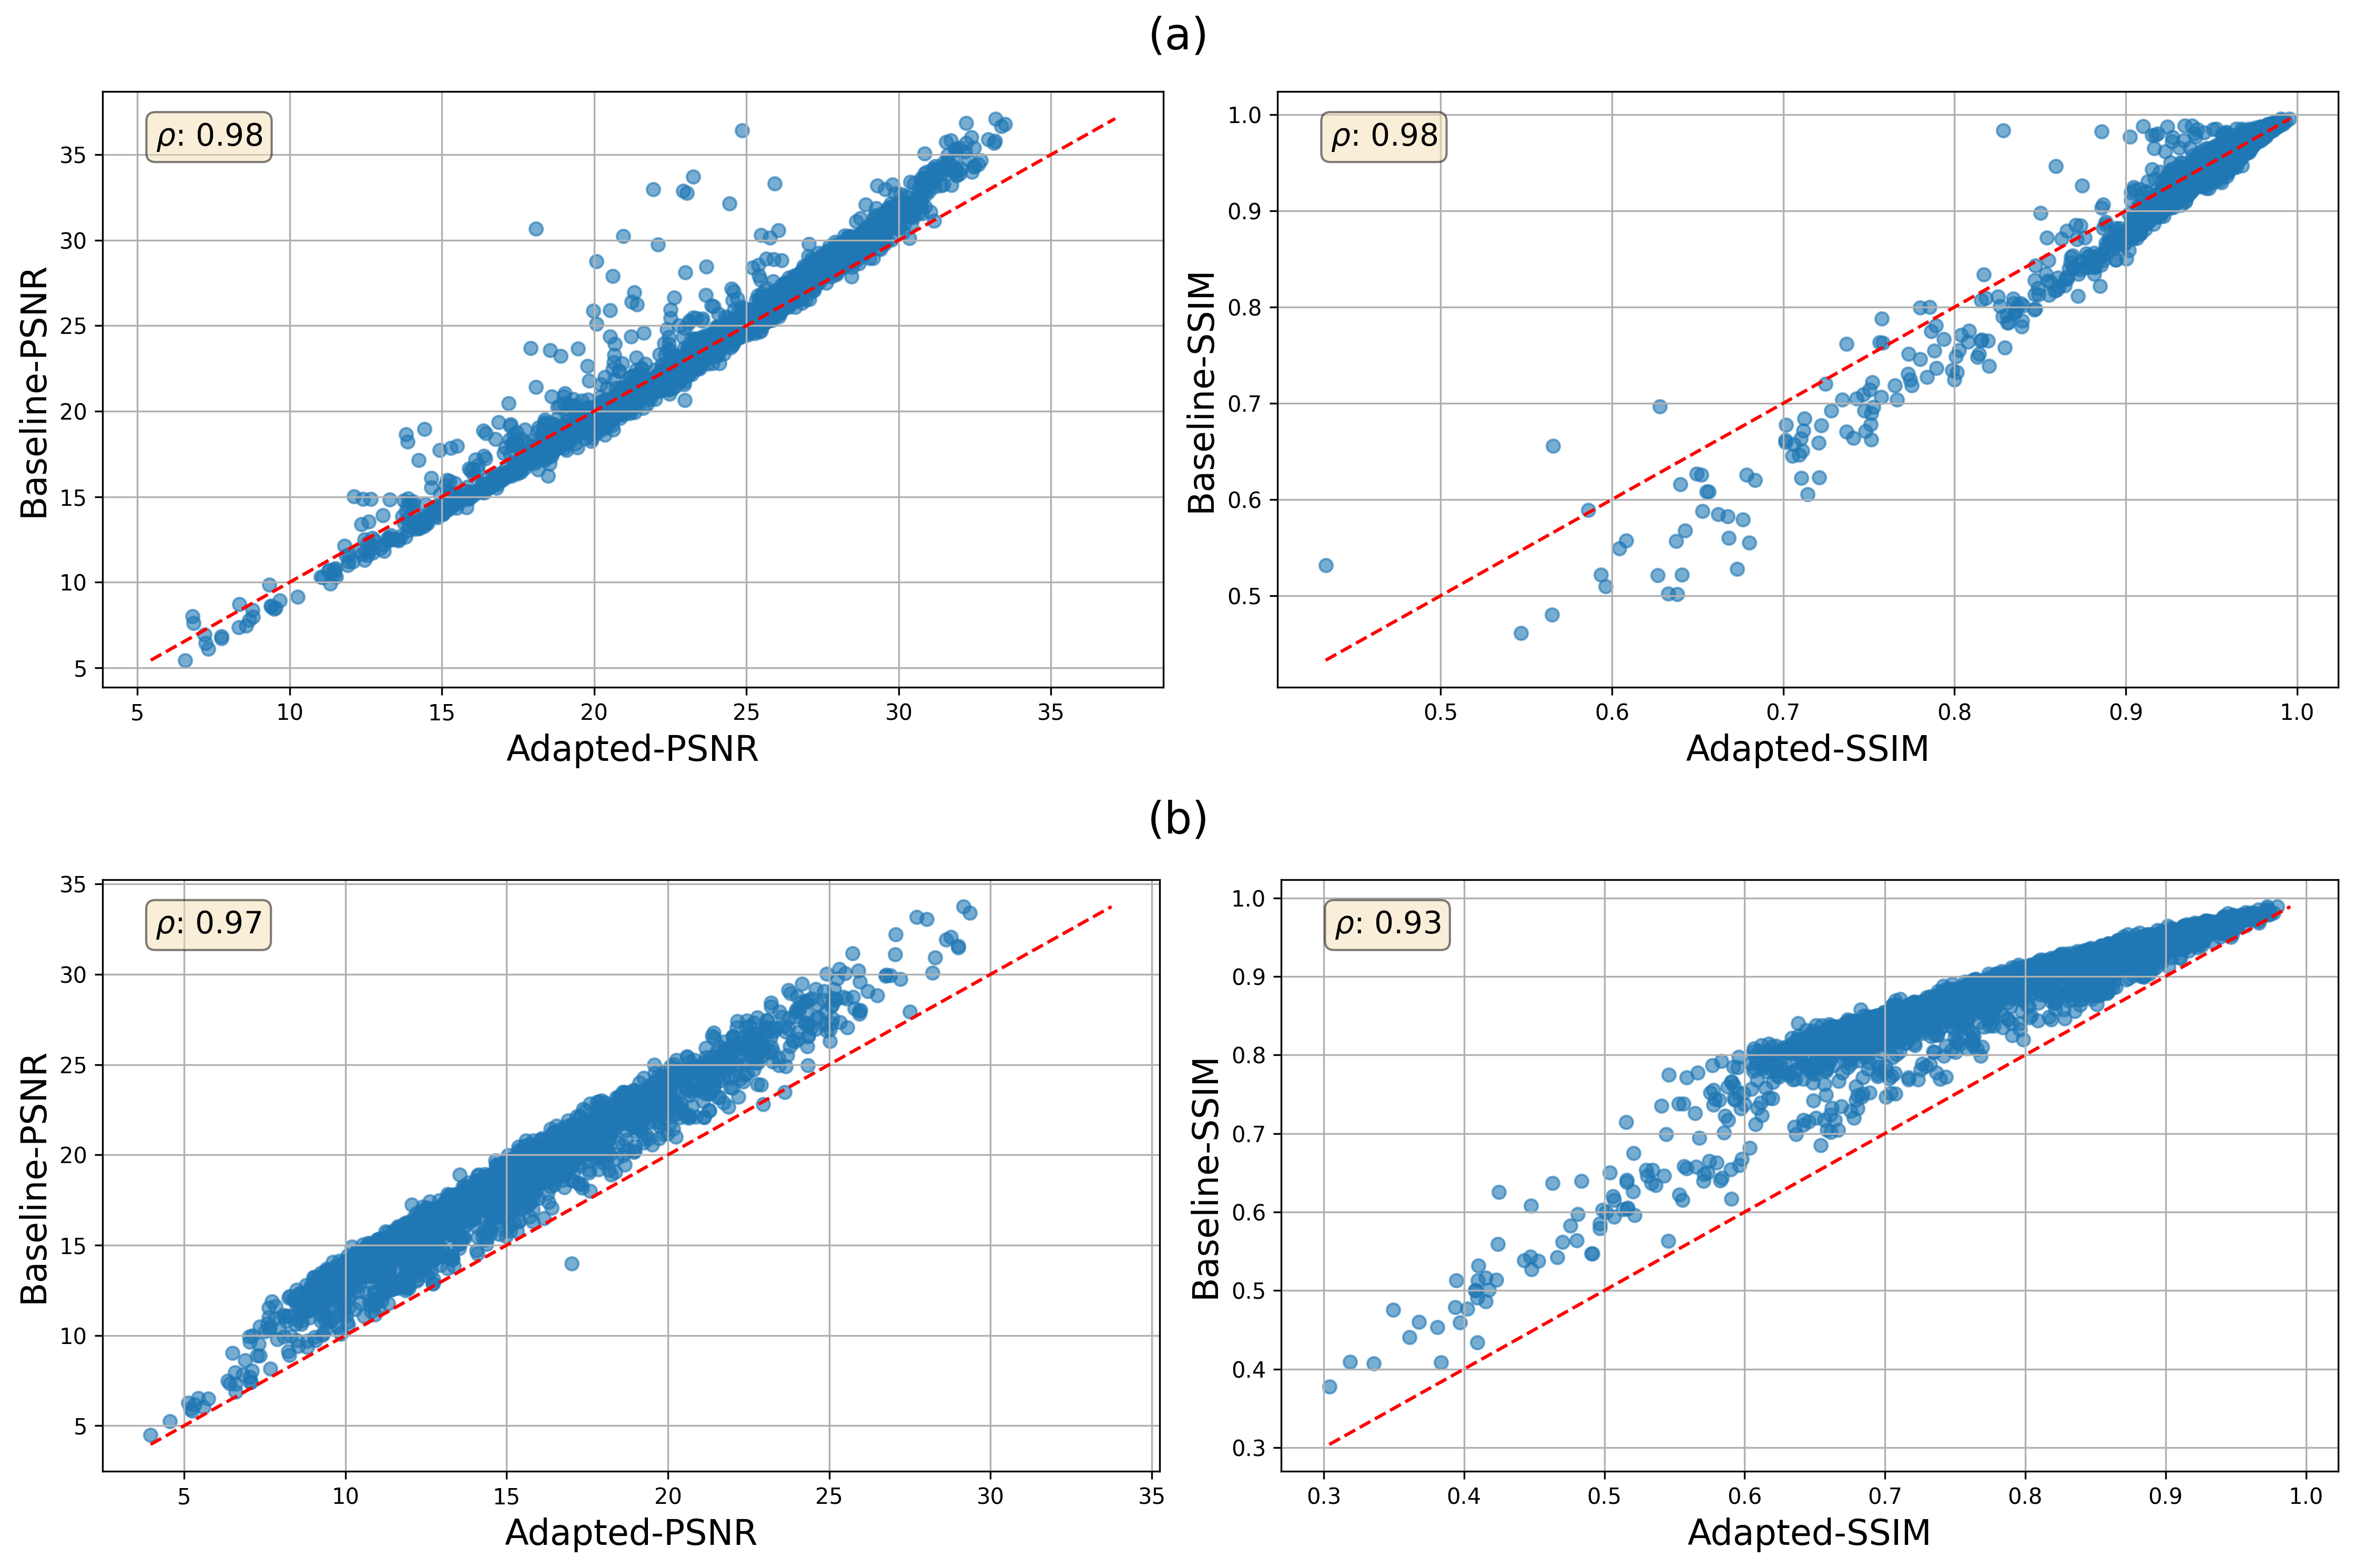
\includegraphics[width=\textwidth]{Includes/5-source-domain-comparison.png}
            \caption{Performance obtained by super resolving the degraded images coming out of the generator. 
                     In (a), the corresponding SR model of each pipeline is used. 
                     In (b), a simple bicubic upsampling is used to super resolve the degraded images. }
            \label{fig:5-source-domain-comparison}
        \end{figure}

        Fig \ref{fig:5-source-domain-comparison} proves the relevance of the domain gap in super resolution, the SR model is able to estimate the inverse of the degradation function in most cases, if given the correct data.
        The problem relies on that in most experiments, the wrong degradation is shown to the model, forcing it to learn the inverse of an incorrect function.  
        This plays an essential role when deploying super resolution model in real production environments, where the degradation model may not be known. 

    \subsection{Target domain}

        This subsection will show the results from the experiments performed on the target domain, which is the equivalent of the red arrows flow described in fig. \ref{fig:3-GAN-degradation-model}.
        In this case, the GAN trained for the degradation model is discarded and only the super resolution model is used.
        The input images are real FOREST-2 images, and the output images are super resolved versions of them. 
        Due to the unpaired nature of the dataset, the performance of the SR model can not be evaluated using metrics like PSNR and SSIM. 
        Other alternatives will be presented, and a qualitative analysis will be performed. 
        Additionally, a quantitative analysis will be discussed using a very small sample of paired data obtained by synchronizing the overpass of FOREST-2 with the route of ECOSTRESS.


        In Fig. \ref{fig:5-target_prediction_sample}, the super resolutions models were used with a 264x264 pixels crop of a real FOREST-2 image.
        The results show that the baseline model, trained with a target domain consisting degraded versions of the synthetic FOREST-2 images ($\mathcal{D}_{\text{SF}-\text{SF}}$), has very similar results as bicubic upsampling.
        On the other side, the adapted model, trained using real FOREST images as the target domain ($\mathcal{D}_{\text{SF}-\text{RF}}$), is able to recover more details, producing sharper images.
        In the frequency domain, the effects of super resolution are clear, as the high frequency components are amplified compared to bicubic upsampling. 
        In this case, the adapted model amplifies frequencies close to the center of the FFT.
        
        


        \begin{figure}[H]
            \centering
            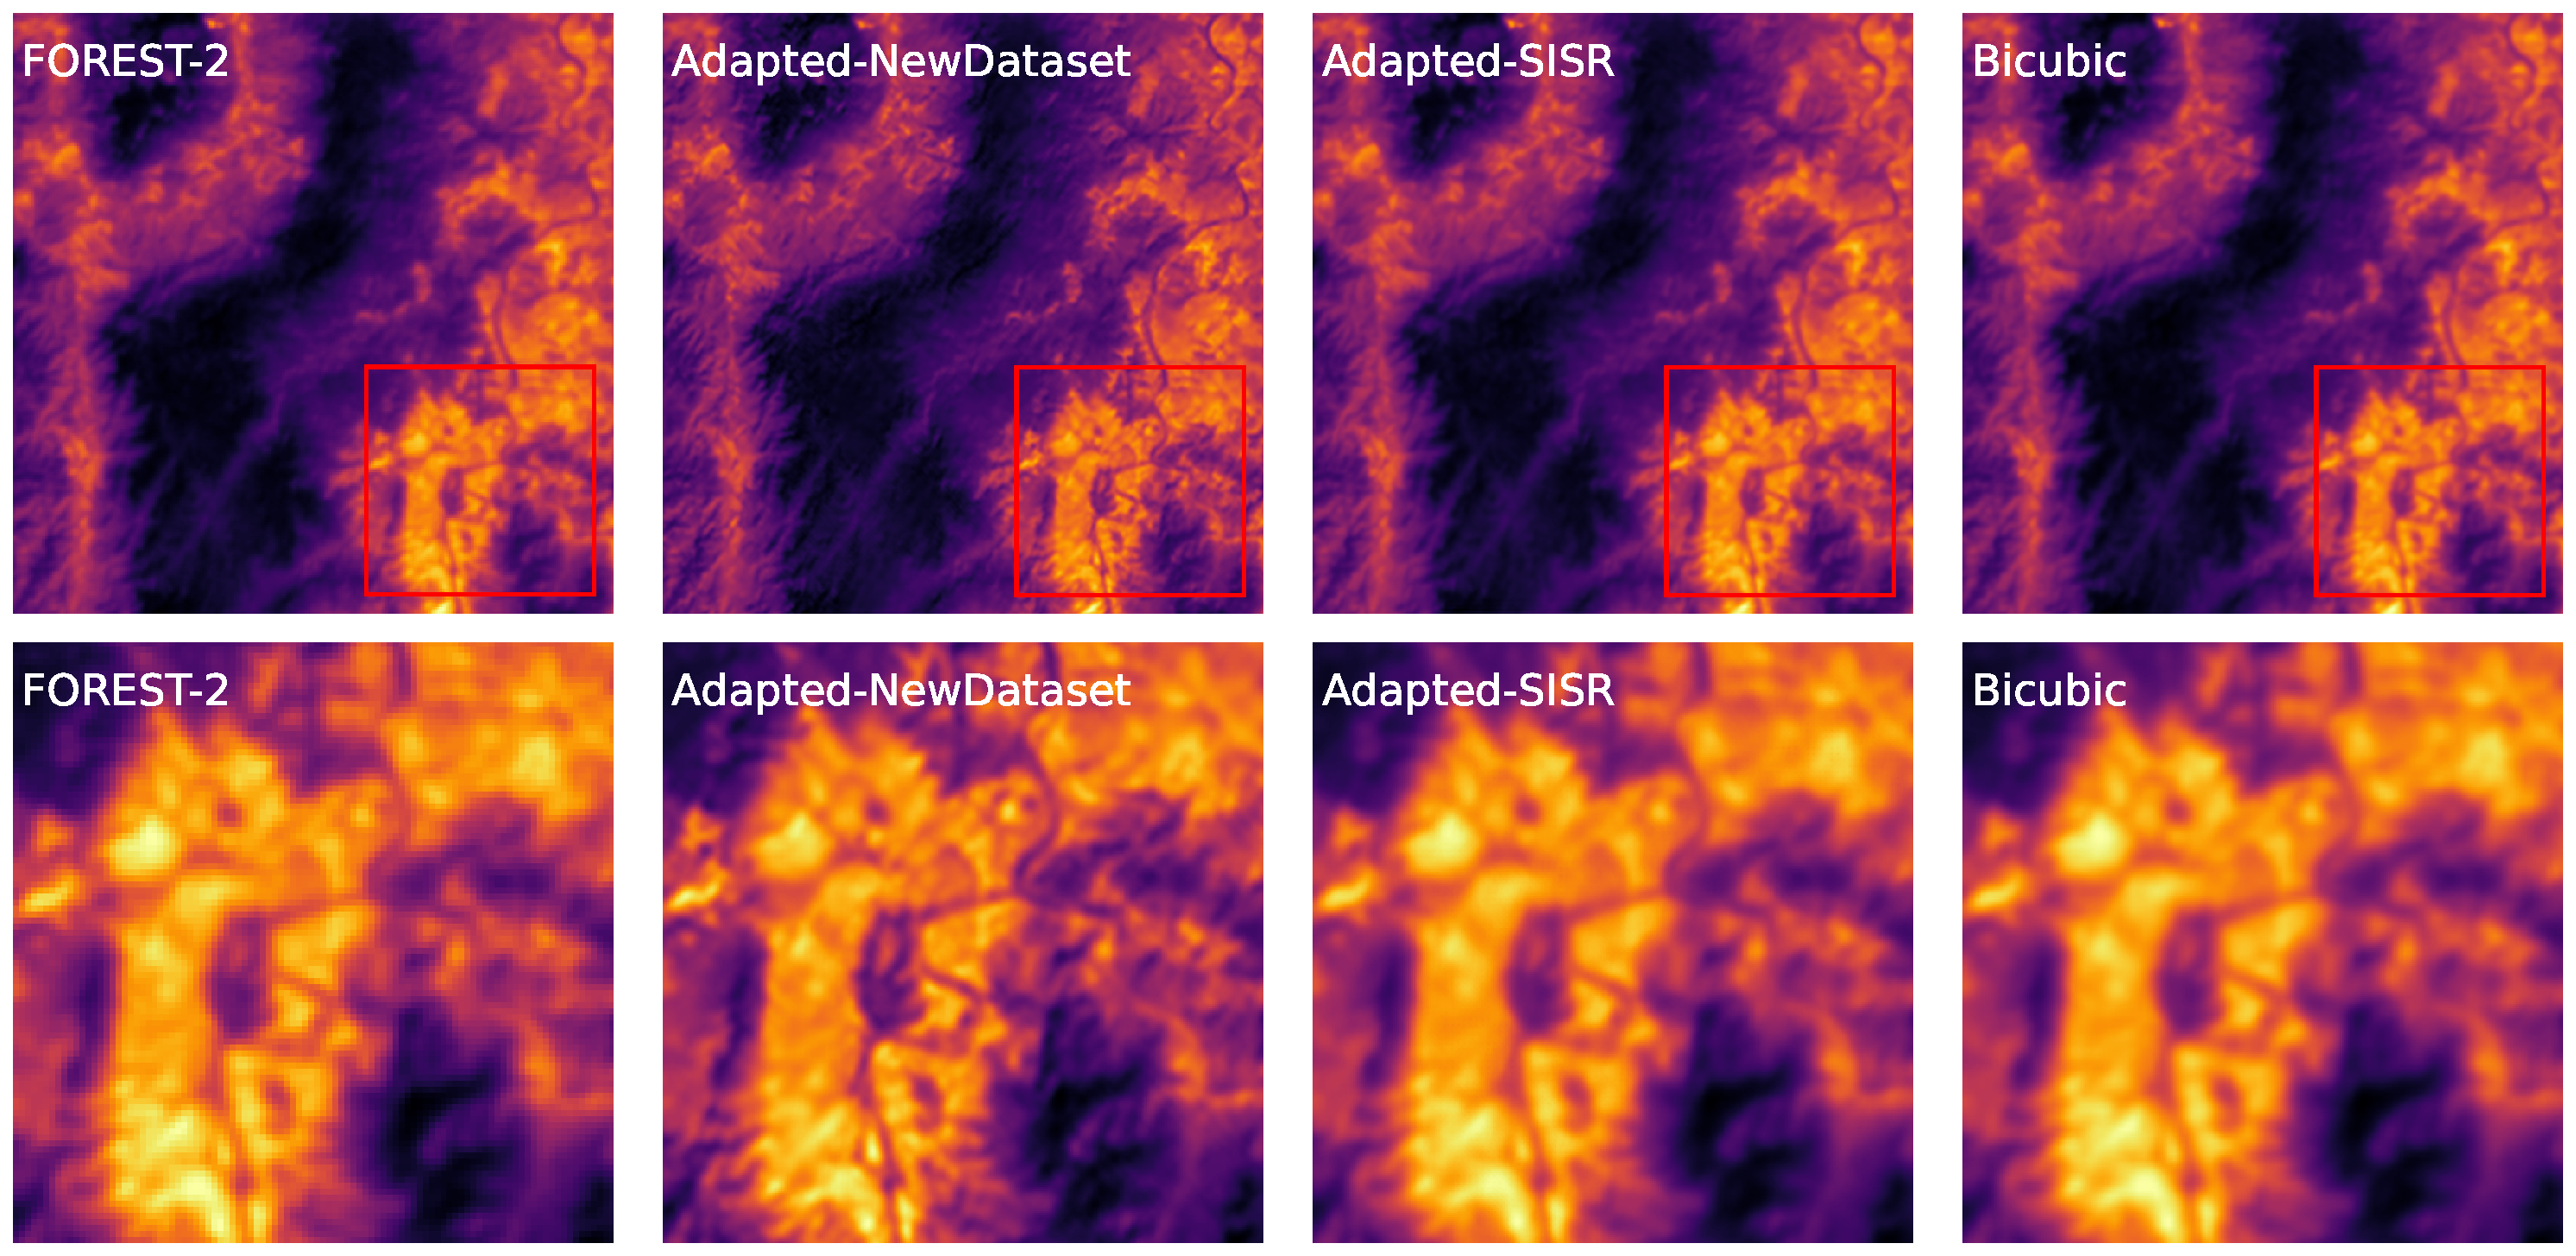
\includegraphics[scale=0.28]{Includes/5-target_prediction_sample.pdf}
            \caption{Super Resolved Forest-2 Scene using different SR models.
                     In the upper row, the image is displayed. A detailed zoom is displayed below. The bottom row shows the log magnitude of the FFT for the images.
                     The original image is displayed in the left, while the super resolved images are displayed afterwards.
                    }
            \label{fig:5-target_prediction_sample}
        \end{figure}

        The results of Fig. \ref{fig:5-target_prediction_sample} with the theory and the results obtained in the source domain.
        The super resolutions task is to estimate the inverse function of the degradation process. 
        When the model is trained using an optimistic degradation process, the model is snot able to recover details from images generated by a more complex degradation process, like the real FOREST-2 images.
        The lack of details in the baseline-SISR images is not because the model is not able to recover them, but because a more optimistic degradation model was used in training. 
        This is an important result to drive the attention to the importance of the degradation model used in training, instead of focusing on more complex super resolution architectures.

        Fig. \ref{fig:5-target-amplification-statistics} shows a more detailed analysis of the frequency domain of the SR images obtained by applying different SR models to the real FOREST-2 validation dataset.
        The upper row shows the log magnitude of the FFT for the SR images of the whole validation dataset, adding ±1 standar deviations to take their variances into account. 
        Up until 0.3 cycles per pixel, the adapted model amplifies the frequencies more than the baseline model, with a similar behaviour afterwards.
        As higher frequencies are related to noise and artifacts, this suggests that the adapted model is able to recover more details than the baseline model, while minimizing undesired components.
        The amplification plot of the SR models against bicubic upsampling shows the same behaviour in a more clear way. Between 0.1 and 0.25 cycles per pixel, the amplification peaks  between 6 and 8 dB on average with respect to bicubic, while the baseline model is between 0 and 2 dB.
        Such amplification, at a pixel size of 70m, corresponds to cycle frequencies between  300 $\frac{1}{m}$ and 700 $\frac{1}{m}$, which is consistent with the loss of components observed in \ref{fig:5-lr-images-fft-comparison}.
        The variability of the amplification allows to conclude that this amplification is consistently higher than the baseline-SISR for all the validation dataset.
        On the other side, while the amplification is very similar in frequencies related to noise, the adapted model seems to step up a little bit compared to the baseline.  
        This suggests that the adapted model is able to recover details from real FOREST-2 images, amplifying frequencies of interests, at the cost of a small increase in the overall noise of the image.

        \begin{figure}[H]
            \centering
            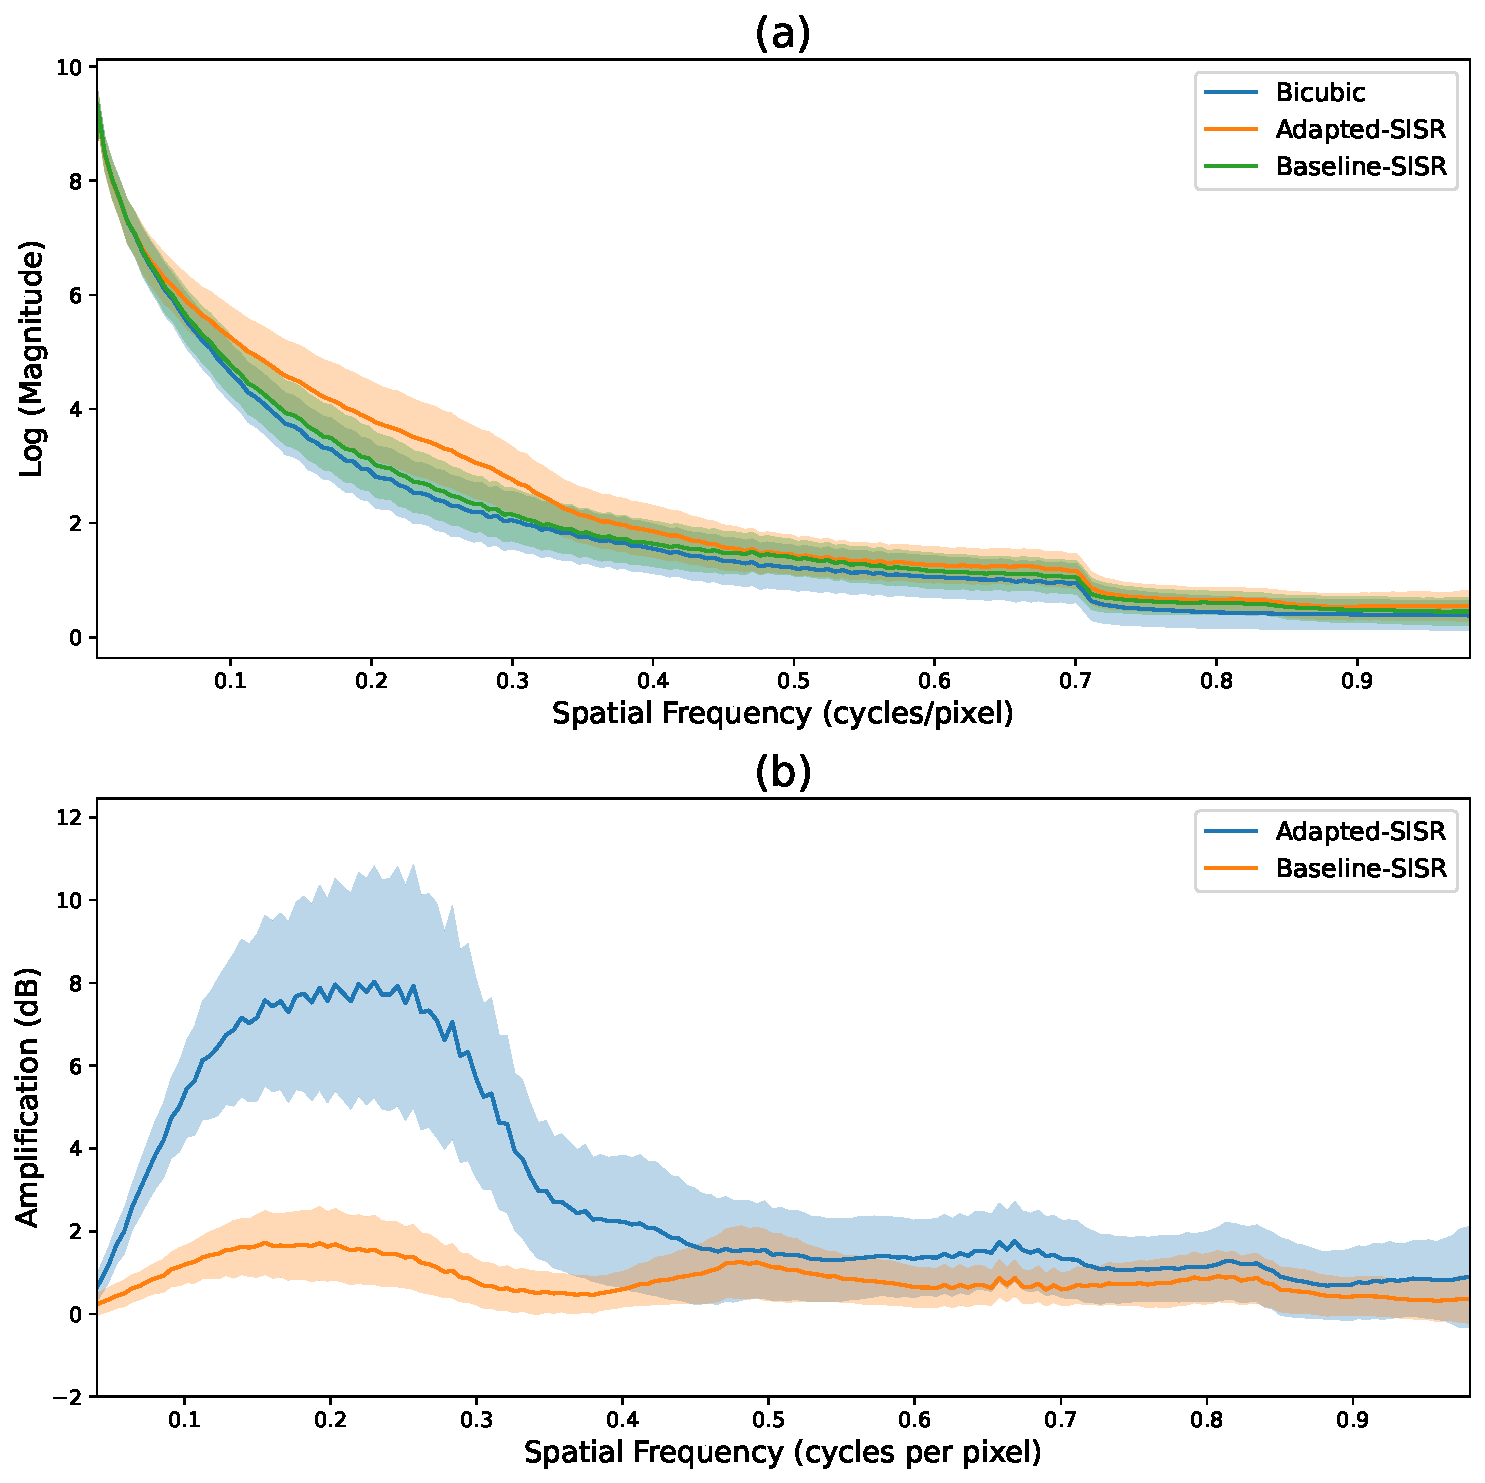
\includegraphics[scale=0.5]{Includes/5-target-amplification-statistics.pdf}
            \caption{Frequency domain analysis of the SR images obtained by applying different SR models to the real FOREST-2 validation dataset.
            In (a), the log of the magnitude of the FFT for the SR images is shown,
            while in (b), the amplification with respect to a  simple bicubic upsampling is displayed.}
            \label{fig:5-target-amplification-statistics}
        \end{figure}


        In Fig. \ref{fig:6-target-gradient-analysis-image}, an example of the gradient analysis of the SR images is shown. 
        Compared to the baseline SISR model, the adapted model shows higher gradient magnitudes, suggesting that the adapted model is able to recover more details than the baseline model. 
        However, in the more dark sections of the gradient magnitude, some small background noise can be percieved, consistent with the results of the frequency domain analysis.

        \begin{figure}[H]
            \centering
            \includegraphics[scale=0.28]{Includes/6-target-gradient-analysis-image.pdf}
            \caption{Gradient analysis of the super resolved images using different SR models for scenes coming from the real FOREST-2 validation dataset.
                     In the upper row, the image is displayed. The gradients in the x and y direction ($G_x$ and $G_y$ respectiely) are displayed below.
                     the gradient magnitude $|G|$ is displayed in the bottom row.}
            \label{fig:6-target-gradient-analysis-image}
        \end{figure}

        Fig \ref{fig:5-gradient-histogram-validation-dataset} shows the distribution frunction of all the gradient magnitudes, estimated through a histogram, for the whole validation dataset.
        Both the adapted and the baseline model show a decrease in the number of pixels with low gradient magnitudes, suggesting that both models are able to recover more details than bicubic upsampling.
        However, the adapted model shows a consistently higher number of pixels with high gradient magnitudes, implying that the adapted model is able to recover more details than the baseline model.
        This is consistent with the observed results and the frequency domain analysis. 
        However, it is important to note that the gradient magnitude is not a good measure of the performance of the SR model, as it does not take into account the noise and artifacts that may be present in the image.
        It represents only a complementary way to understand the effects of the SR model.


        \begin{figure}[H]
            \centering
            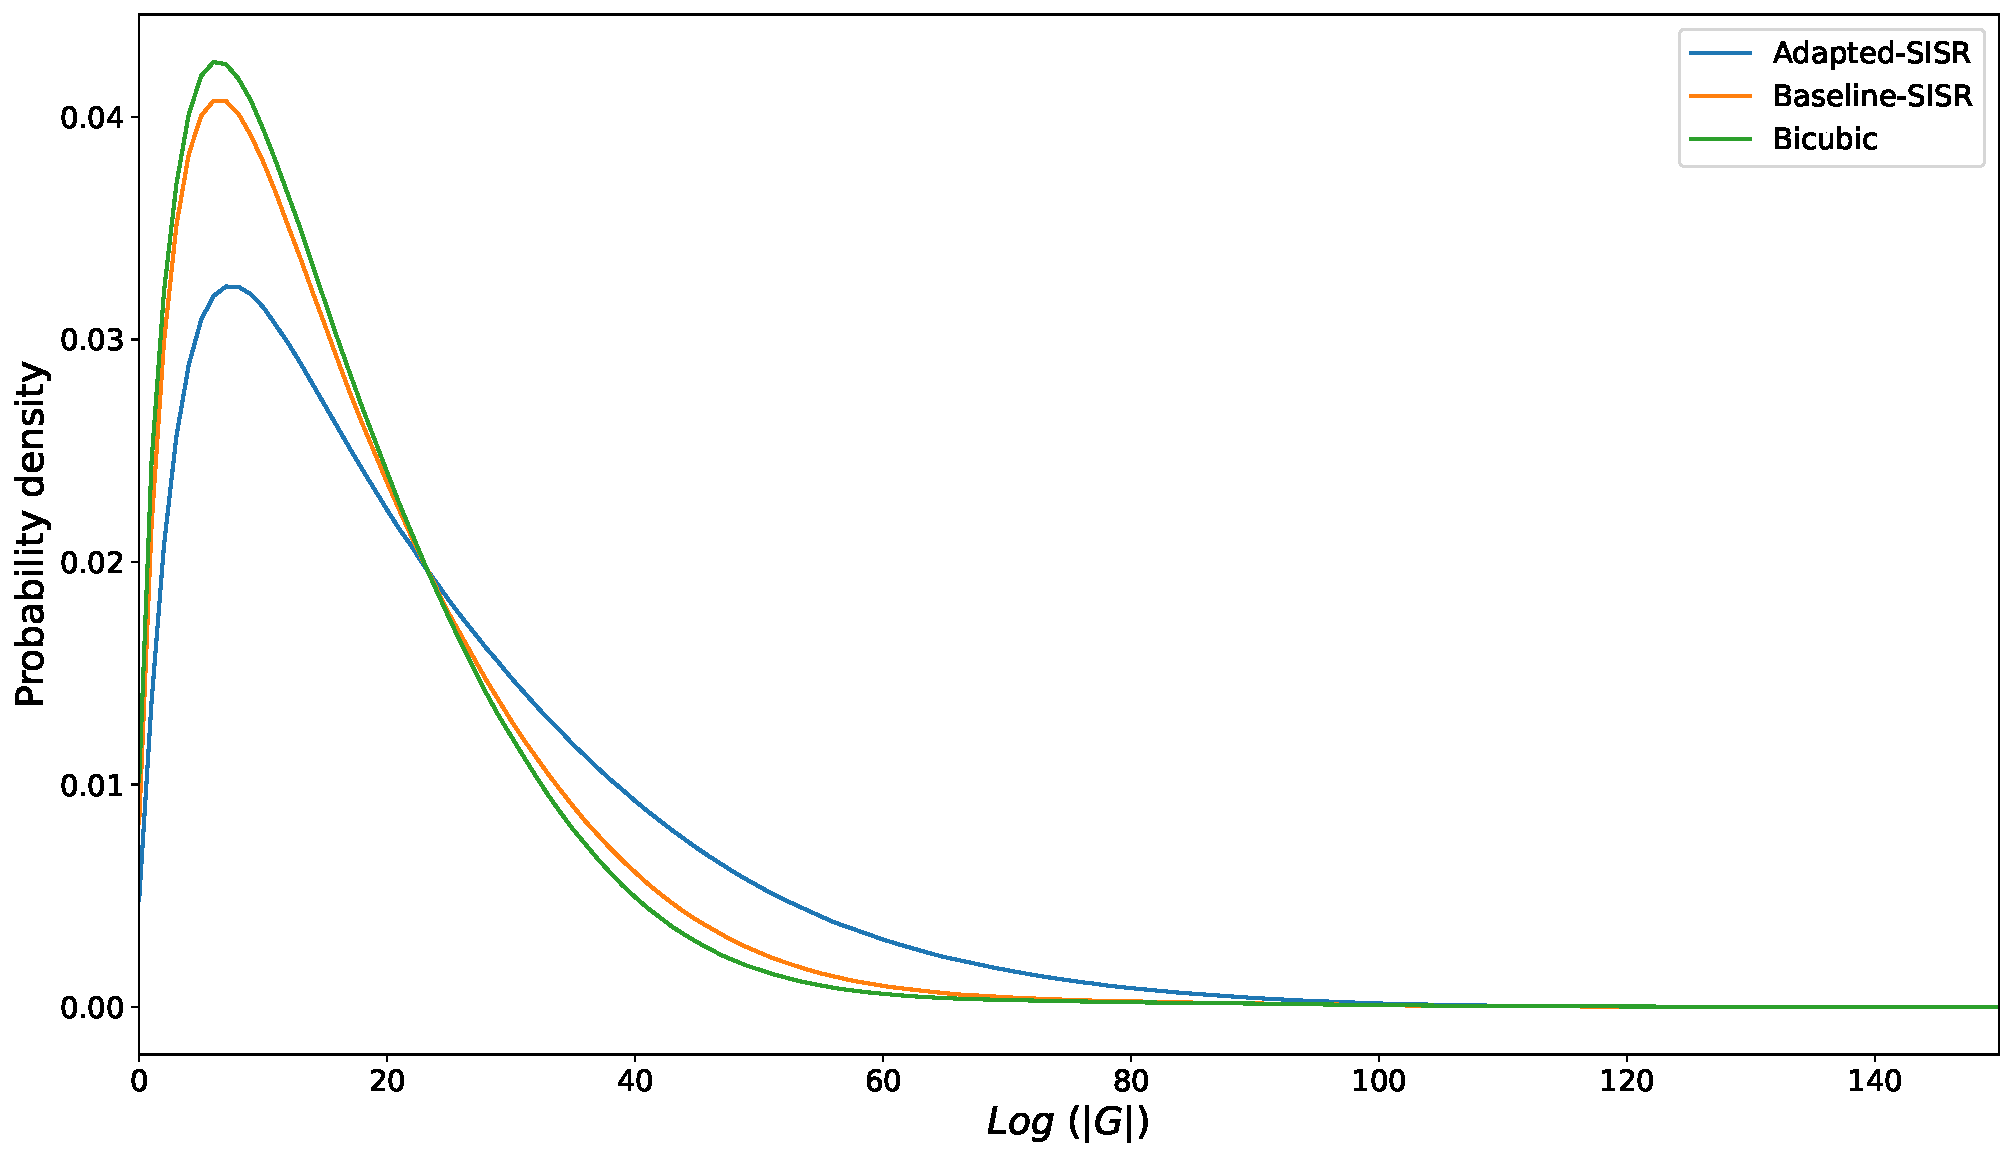
\includegraphics[scale=0.4]{Includes/5-gradient-histogram-validation-dataset.pdf}
            \caption{Histogram of the gradient magnitude $|G|$ for the whole validation real FOREST-2 dataset.}
            \label{fig:5-gradient-histogram-validation-dataset}
        \end{figure}

    \subsection{Effects of the domain gap}

        The combination of the probabilistic degradation model and the SR model were proven helpful to bridge the domain gap and inprove the resolution of real FOREST-2 images.
        However, it is important to understand what happens when the target domain used in training does not match the conditions that will occur in the real world.
        Two situations are identified, the first one is when the target domain used in training is more complex than what will be used in production, and the second one is when the target domain used in training is simpler than what will be used in production.
        The latter was largely adressed in this work, when the HR-LR pairs are generated using a baseline degradation model, which is overly optimistic. 
        Another example of it would be that images taken from FOREST-2 in several years may not have the same distribution as current images, as the instruments may have degraded over time.
        However, the first one was not addressed, and is the focus of this subsection.
        
        To simulate this situation, the model trained using real FOREST-2 images was used to super resolve synthetic FOREST images degraded using the baseline degradation model.
        The results are shown in Figs. \ref{fig:5-target-prediction-with-domain-gap} and \ref{fig:5-target-prediction-with-domain-gap-fft}.
        The performance of the adapted model is catastrophic, producing several artifacts and yielding a PSNR difference of approximately 10dB, which represent a 10x difference in terms of MSE.

        \begin{figure}[H]
            \centering
            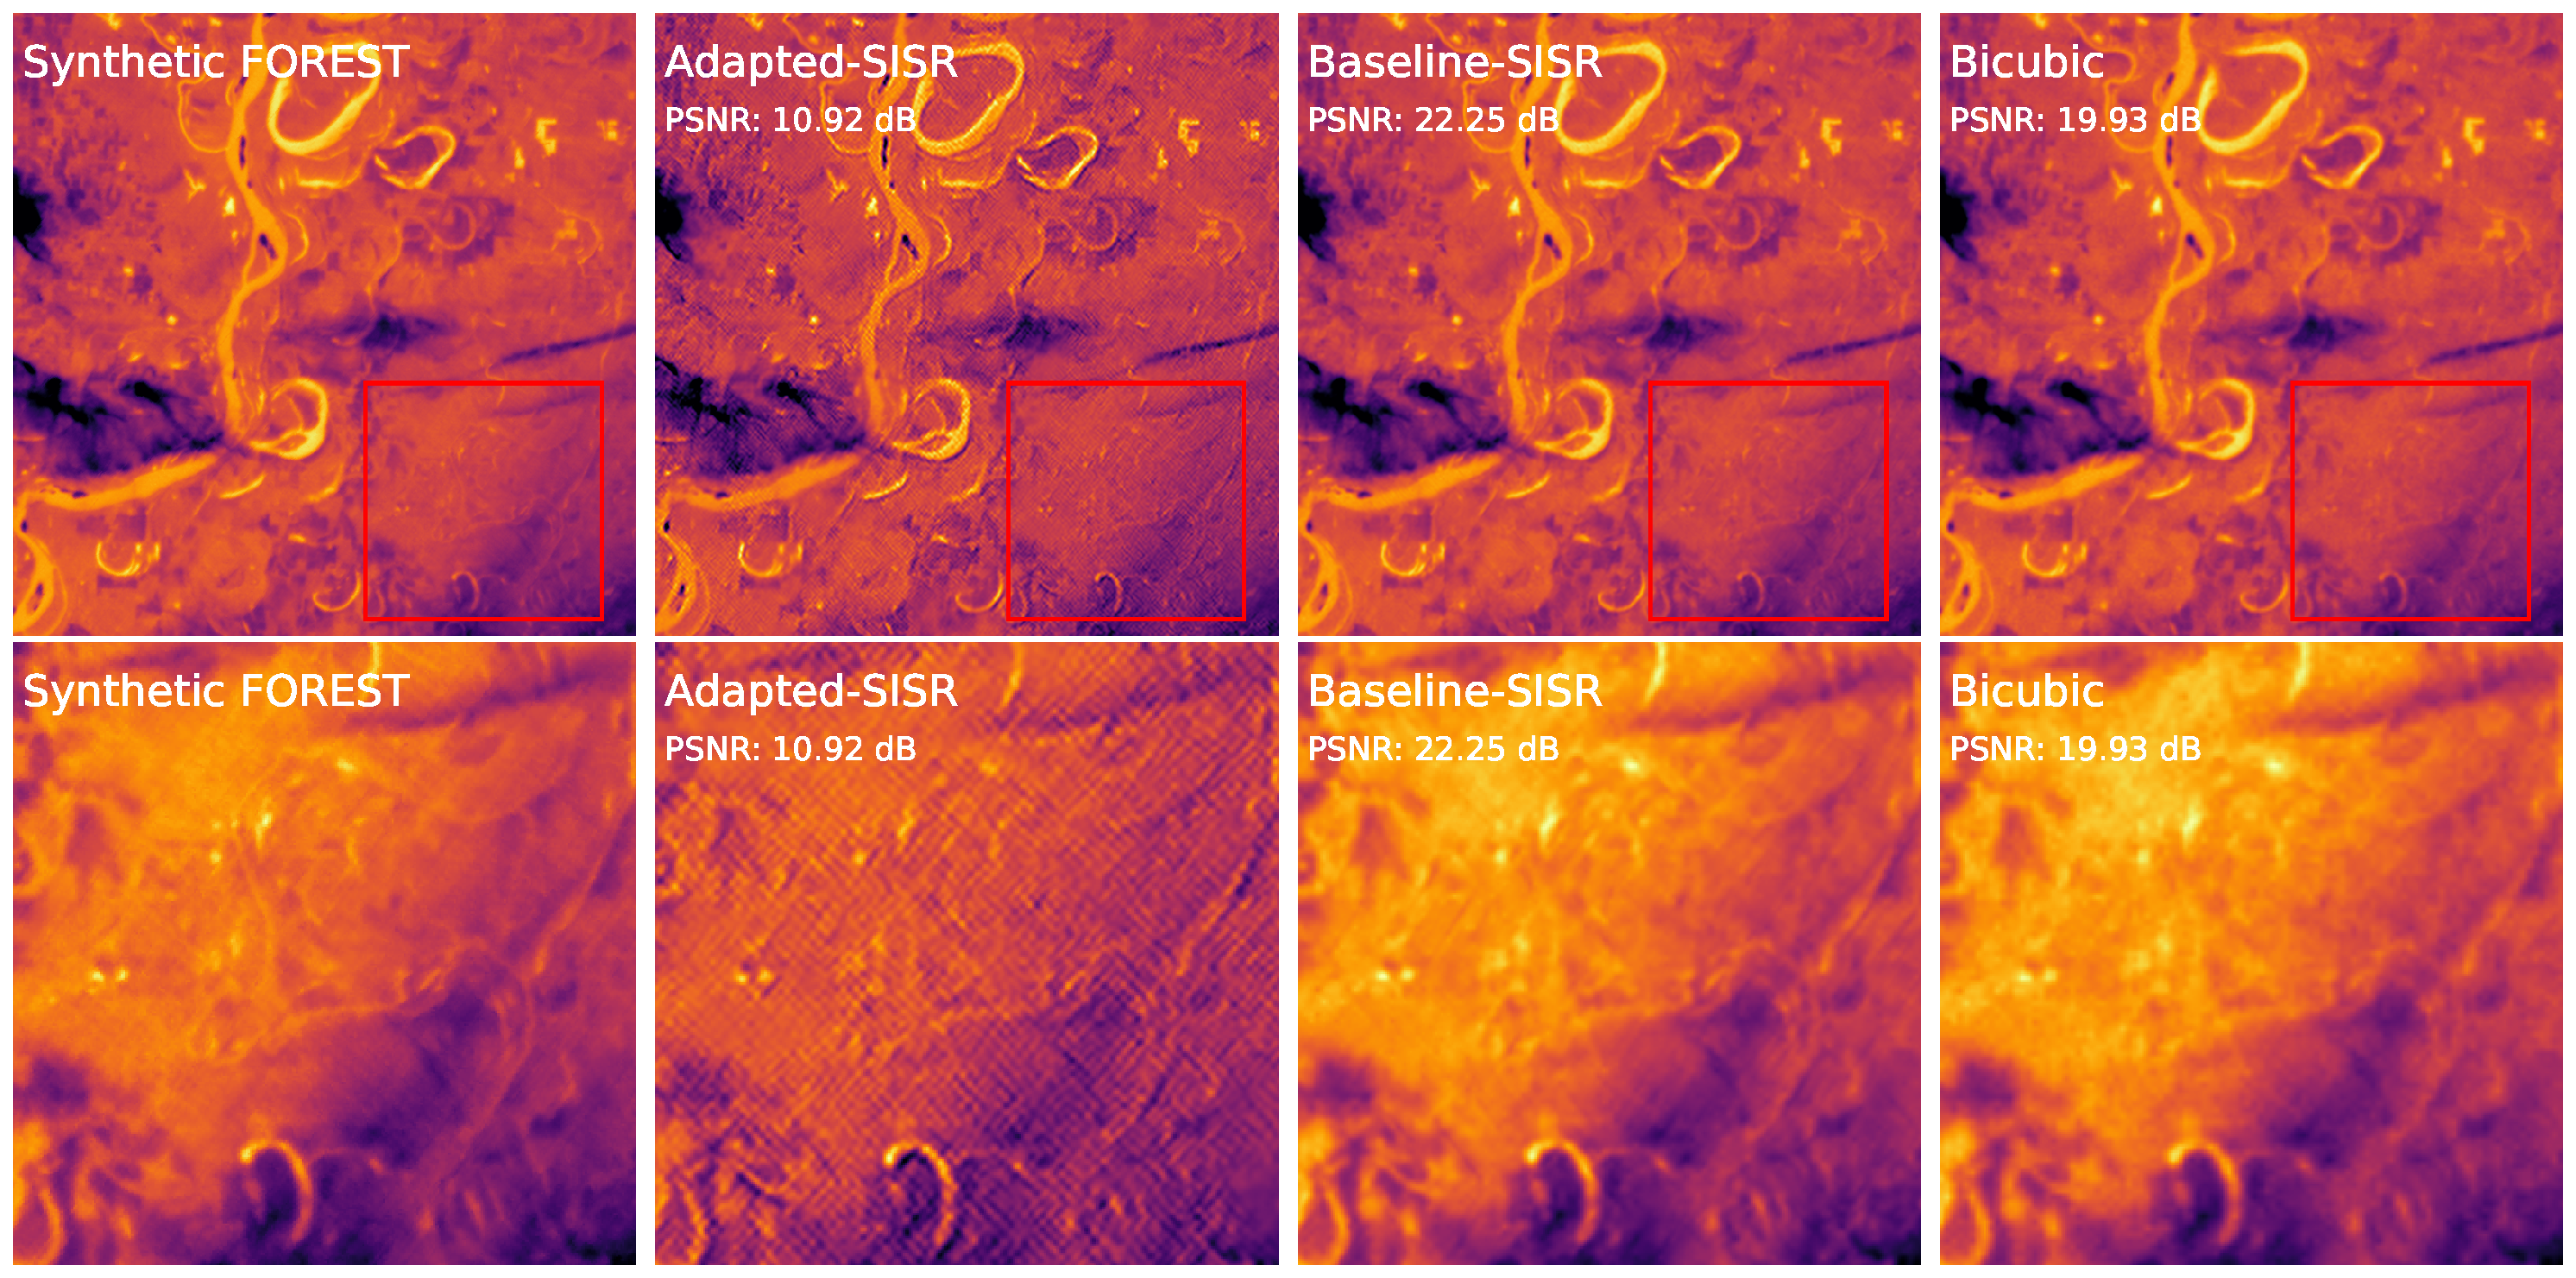
\includegraphics[scale=0.28]{Includes/5-target-prediction-with-domain-gap.pdf}
            \caption{Effects of using a model trained with on different domain than at inference time. 
                     When using an Synthetic FOREST image degraded with the baseline degradation model as an input, the model trained using real FOREST-2 data as the target domain generates several artifacts and underperforms severly in terms of PSNR. }
            \label{fig:5-target-prediction-with-domain-gap}
        \end{figure}

        In the frequency domain, the results  are shown in Fig. \ref{fig:5-target-prediction-with-domain-gap-fft}.  
        The adapted model adds amplification in the higher range of spatial frequency, related with noise and artifacts. The frequencies related to the proper signal are also amplified, suggesting an improvement in the resolution.
        This suggests that while the adapted model highlights edges and details, it also severly amplifies the noise and artifacts, resulting in a worse performance in terms of PSNR.
        It is important to note that the amplification curve does not show a considerable difference with respect to the one in Fig. \ref{fig:5-target-amplification-statistics},
        highlighting the fact that the frequency analysis is not suitable by itself to evaluate the performance of the SR model.

        \begin{figure}[H]
            \centering
            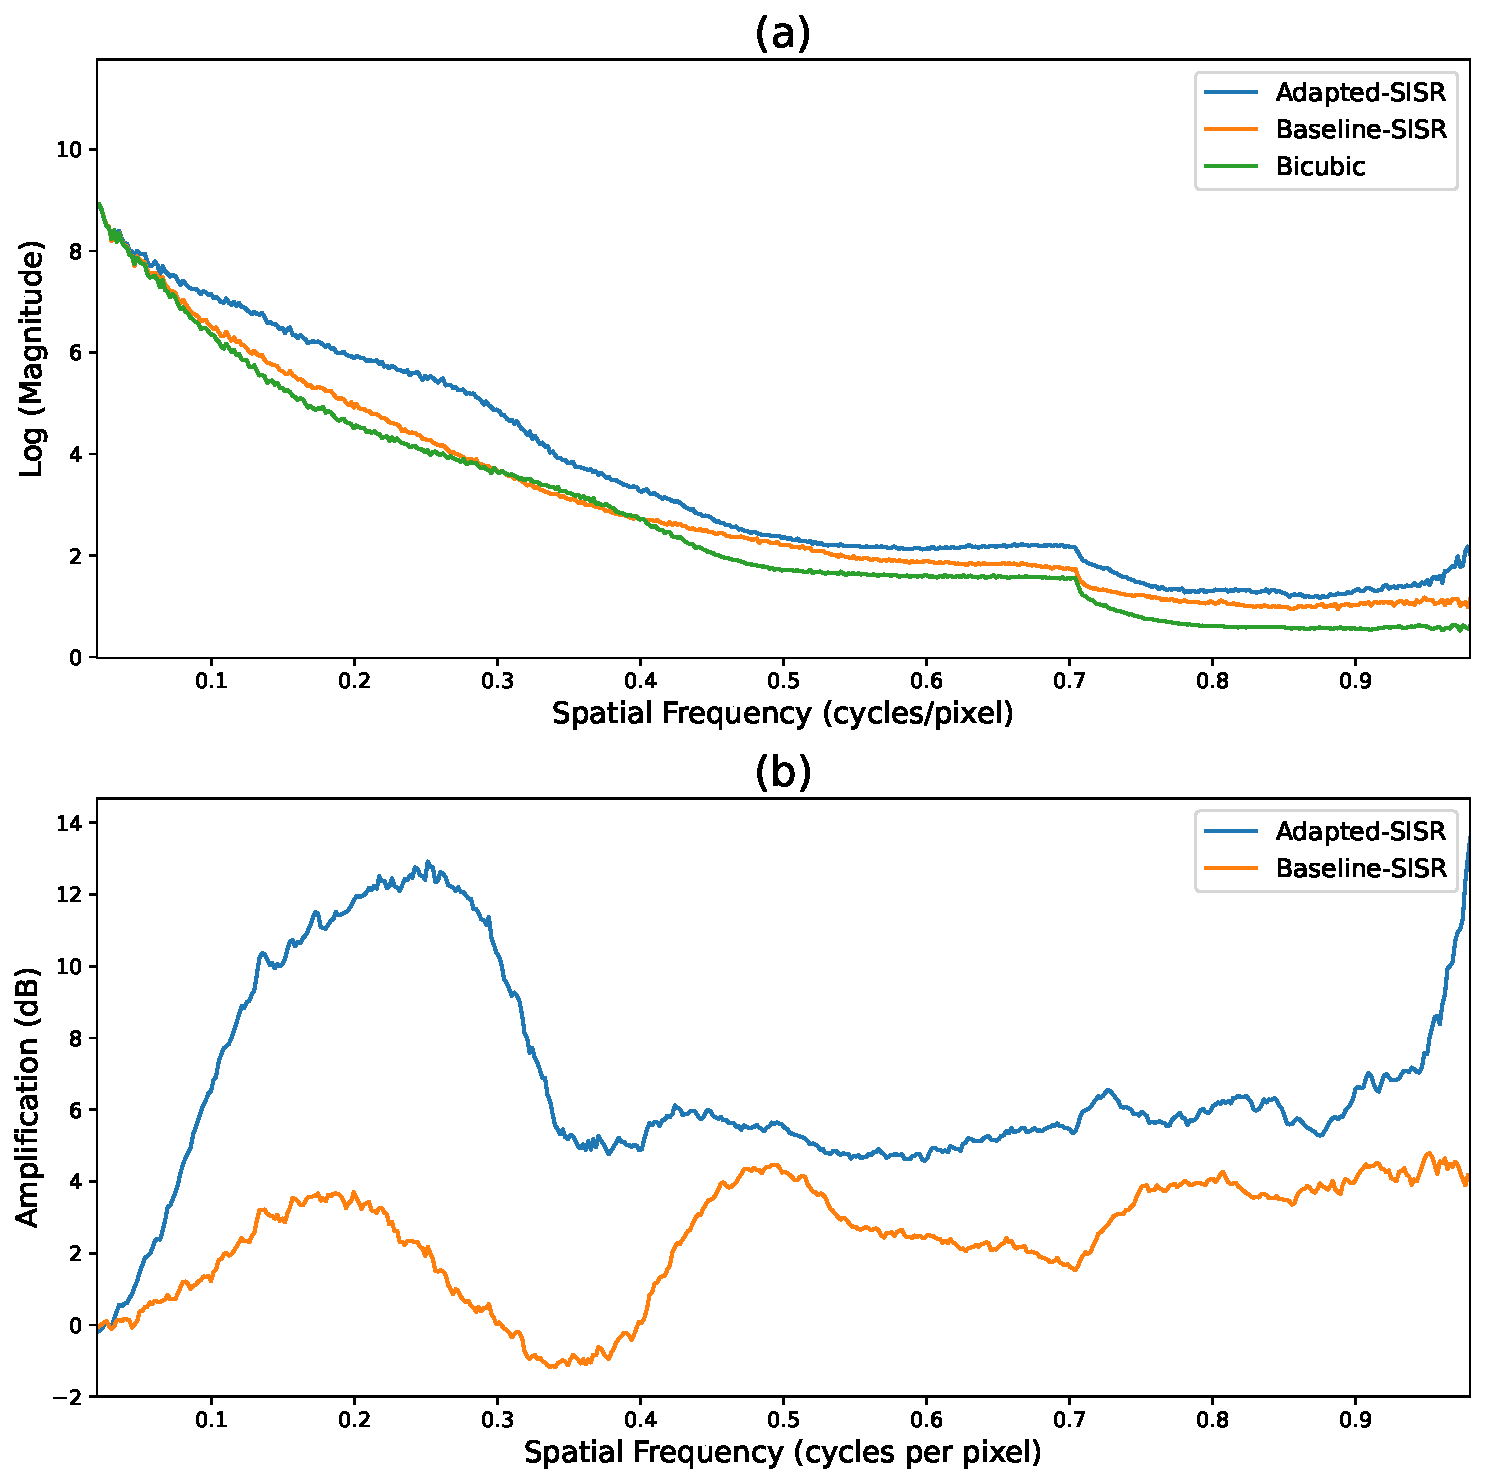
\includegraphics[scale=0.4]{Includes/5-target-prediction-with-domain-gap-fft.pdf}
            \caption{Effects of using a model trained with on different domain than at inference time. 
                     (a) shows the log magnitude of the radial average of the FFT for the SR images using different algorithms.
                     (b) shows the amplification with respect to bicubic interpolation
                     }
            \label{fig:5-target-prediction-with-domain-gap-fft}

        The performance results in terms of different metrics are shown in Fig. \ref{fig:5-target-prediction-with-domain-gap-dataset}. 
        In the conditions described above, the adapted super resolution model underperforms severly considered metric.


        \begin{figure}[H]
            \centering
            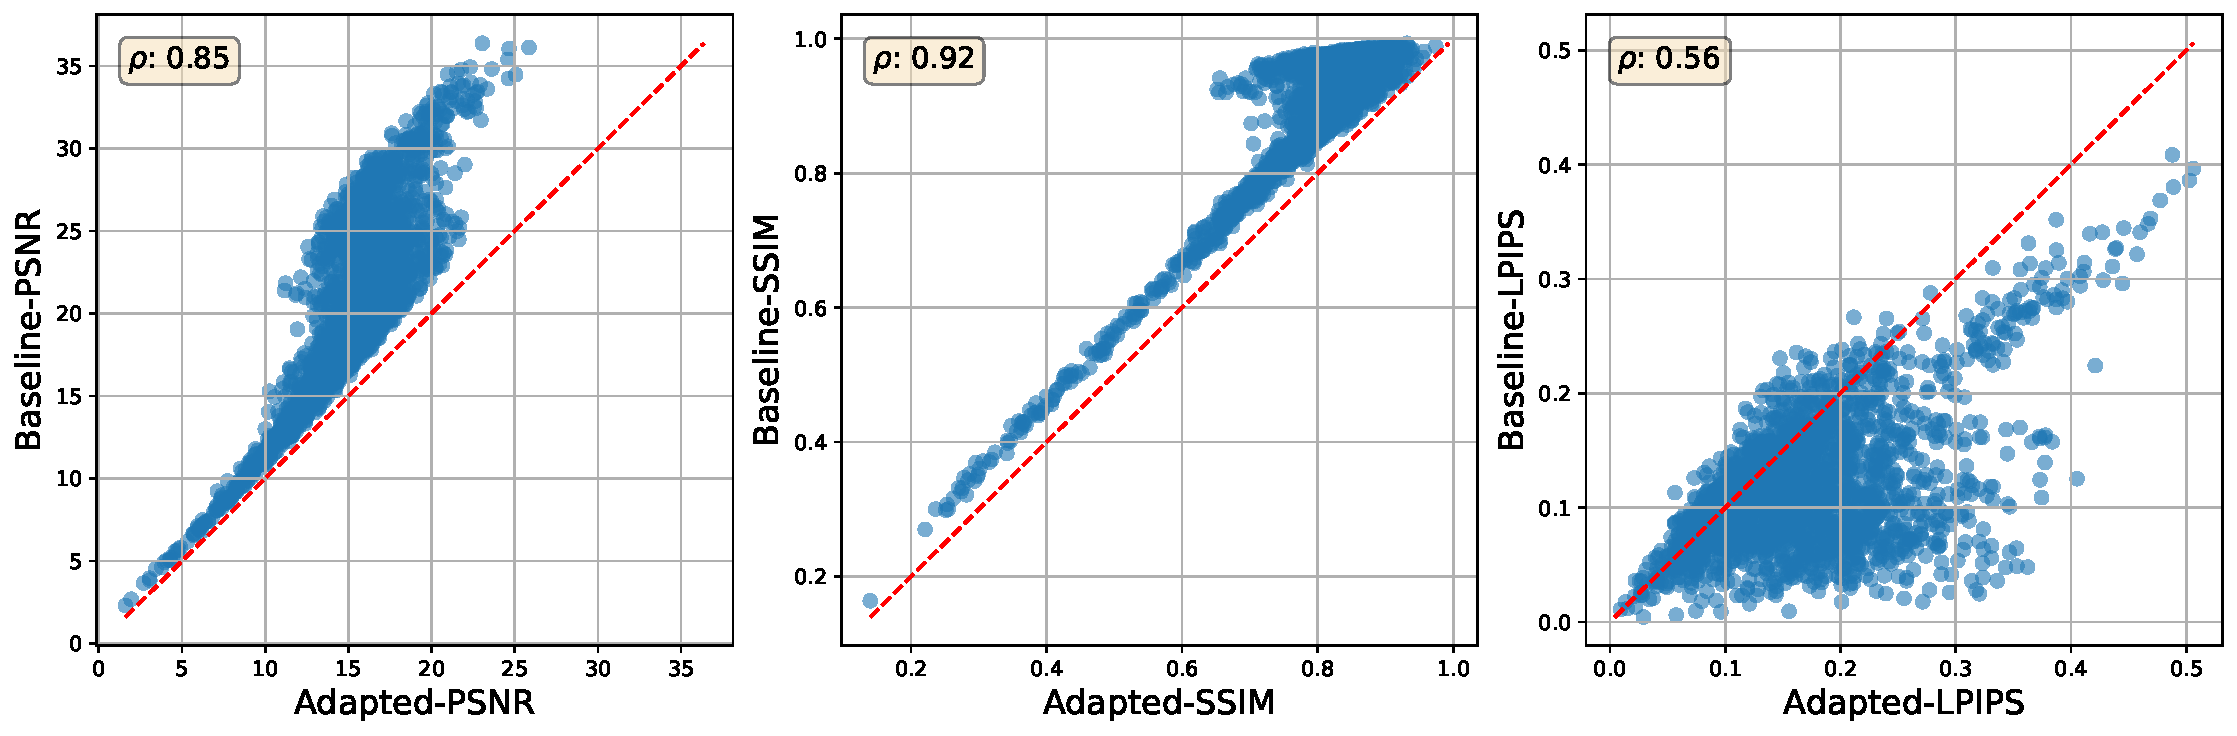
\includegraphics[scale=0.38]{Includes/5-target-prediction-with-domain-gap-dataset.pdf}
            \caption{Performance obtained by super resolving the degraded synthetic FOREST images using different super resolution models.}
            \label{fig:5-target-prediction-with-domain-gap-dataset}
        \end{figure}


        


        \end{figure}

        
        
    This demonstrates that while this approach is very good to bridge a domain gap, it is not robust at all to domain shifts. 
    This limitation is in sync with what is found in the literature, where GAN approaches are not able to generalize to arbitrary domains DASDASD.


    As in the target domain the ground truth is not known due to the lack of a paired dataset, the performance of the SR model can not be evaluated using metrics like PSNR and SSIM.
    The result of the image quality assessment metrics were done by super resolving images coming from real FOREST-2 and also from the degraded synthetic FOREST-2 images and calculating their NIQE and BRISQUE scores.
    The results are shown in Fig. \ref{fig:5-target-iqa-results}.
    For both metrics, a large gap is observed between the adapted model and the rest, when the input images come from real FOREST-2 images. 
    Suggesting that the adapted model is able to produce more natural images than the rest.
    This behaviour does not exactly replicates when the input images come from synthetic FOREST-2 images, where the adapted model is not able to produce more natural images than the rest.
    Moreover, for the adapted model, both metrics tend to get worse when the input images come from synthetic FOREST-2 images. The contrary happens for the rest of the models.
    This suggests that the adapted model is able to produce more natural images than the rest, but only when the input images come from the same distribution as the target domain used in training.
    However, it is important to note that: 

    \begin{enumerate}
        \item The images used for training the NIQE and BRISQUE models are not remote sensing images, and therefore, the results may not be representative. This could be circumvented by training a NIQE/BRISQUE model using remote sensing images only.
        \item NIQE and BRISQUE are objective measures of image quality, not of physical consistency or image fidelity.
    \end{enumerate}

    While the comparison of results may help to understand the behaviour of the models, it is important to note that the results are not representative of the real world performance of the models. 

        \begin{figure}[H]
            \centering
            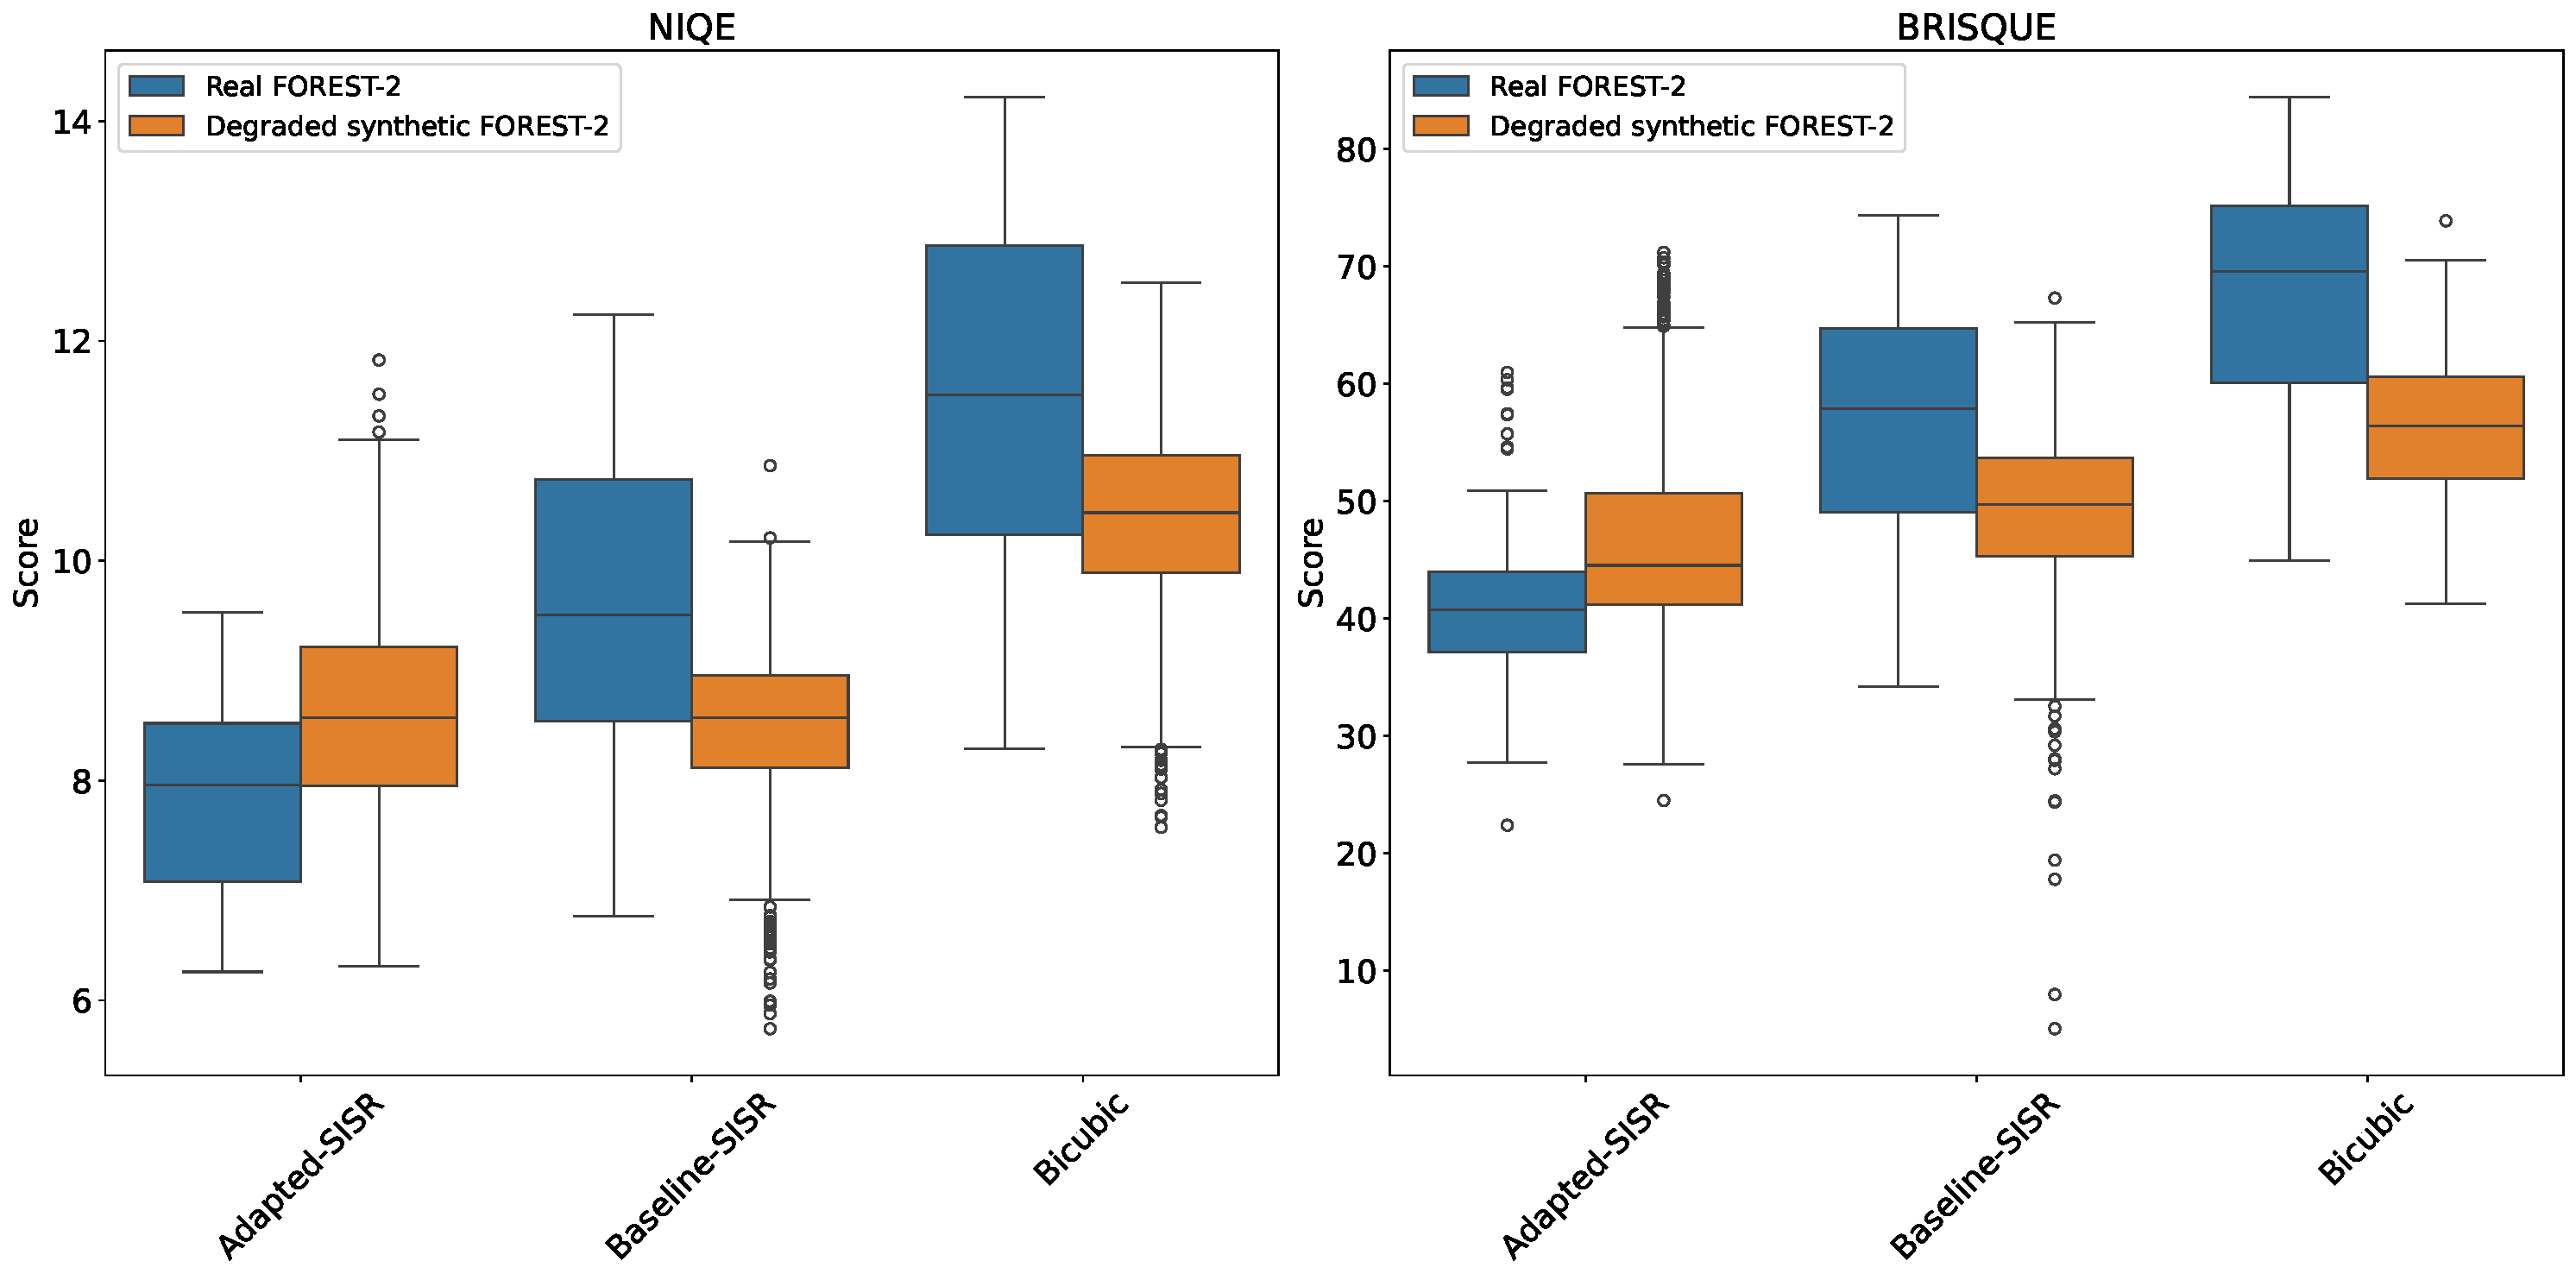
\includegraphics[scale=0.28]{Includes/5-target-iqa-results.pdf}
            \caption{Image quality assessment metrics for the different SR models using different datasets as input. 
                    In both metrics, the lower the score, the better the image quality.}
            \label{fig:5-target-iqa-results}
        \end{figure}


        

        
\newpage
    